%% abtex2-modelo-artigo.tex, v-1.9.7 laurocesar
%% Copyright 2012-2018 by abnTeX2 group at http://www.abntex.net.br/ 
%%
%% This work may be distributed and/or modified under the
%% conditions of the LaTeX Project Public License, either version 1.3
%% of this license or (at your option) any later version.
%% The latest version of this license is in
%%   http://www.latex-project.org/lppl.txt
%% and version 1.3 or later is part of all distributions of LaTeX
%% version 2005/12/01 or later.
%%
%% This work has the LPPL maintenance status `maintained'.
%% 
%% The Current Maintainer of this work is the abnTeX2 team, led
%% by Lauro César Araujo. Further information are available on 
%% http://www.abntex.net.br/
%%
% ------------------------------------------------------------------------
% ------------------------------------------------------------------------
% abnTeX2: Modelo de Artigo Acadêmico em conformidade com
% ABNT NBR 6022:2018: Informação e documentação - Artigo em publicação 
% periódica científica - Apresentação
% ------------------------------------------------------------------------
% ------------------------------------------------------------------------

\documentclass[
	% -- opções da classe memoir --
	article,			% indica que é um artigo acadêmico
	12pt,				% tamanho da fonte
	oneside,			% para impressão apenas no recto. Oposto a twoside
	a4paper,			% tamanho do papel. 
	% -- opções da classe abntex2 --
	% chapter=TITLE,		% títulos de capítulos convertidos em letras maiúsculas
	% section=TITLE,		% títulos de seções convertidos em letras maiúsculas
	% subsection=TITLE,	% títulos de subseções convertidos em letras maiúsculas
	% subsubsection=TITLE % títulos de subsubseções convertidos em letras maiúsculas
	% -- opções do pacote babel --
    BIBLATEX,           % indica para utilizar BIBLATEX em vez do abntex2cite
	english,			% idioma adicional para hifenização
	brazil,				% o último idioma é o principal do documento
	sumario=tradicional
	]{abntex2}

% ---
% PACOTES
% ---
% =============================================================================
% PACOTES E CONFIGURAÇÕES
% =============================================================================

% ---
% Pacotes fundamentais 
% ---
\usepackage{sbc-template}
\usepackage{times}			% Usa a fonte Times new Roman
\usepackage[T1]{fontenc}		% Selecao de codigos de fonte.
\usepackage[utf8]{inputenc}		% Codificacao do documento (conversão automática dos acentos)
\usepackage{indentfirst}		% Indenta o primeiro parágrafo de cada seção.
\usepackage{nomencl} 			% Lista de simbolos
\usepackage{color}				% Controle das cores
\usepackage{graphicx}			% Inclusão de gráficos
\usepackage{microtype} 			% para melhorias de justificação
\usepackage{tikz}               % para ticks
\usepackage{longtable}          % para quebra de tabela por página
\usepackage{tabularray}         % formatação da coluna e linha da tabela
\usepackage{graphicx}           % utilizado para formatação de tabelas
\usepackage{subcaption}         % para subFiguras
% ---
		
% ---
% Pacotes adicionais, usados apenas no âmbito do Modelo Canônico do abnteX2
% ---
\usepackage{lipsum}				% para geração de dummy text
% ---
		
% ---
% Pacotes de citações
% ---
\usepackage[brazilian,hyperpageref]{backref}	 % Paginas com as citações na bibl
\usepackage[alf]{abntex2cite}	% Citações padrão ABNT
% ---

% Pacotes instalados por nós alunos
\usepackage{xurl}

% ---
% Configurações do pacote backref e formatação
% ---
% =============================================================================
% CONFIGURAÇÕES DE FORMATAÇÃO E BACKREF
% =============================================================================

% ---
% Configurações do pacote backref
% Usado sem a opção hyperpageref de backref
\renewcommand{\backrefpagesname}{Citado na(s) página(s):~}
% Texto padrão antes do número das páginas
\renewcommand{\backref}{}
% Define os textos da citação
\renewcommand*{\backrefalt}[4]{
	\ifcase #1 %
		Nenhuma citação no texto.%
	\or
		Citado na página #2.%
	\else
		%Citado #1 vezes nas páginas #2.%
        Citado nas páginas #2.%
	\fi}%
% ---

% ---
% Configurações de aparência do PDF final

% alterando o aspecto da cor azul
\definecolor{blue}{RGB}{41,5,195}

% informações do PDF
\makeatletter
\hypersetup{
     	%pagebackref=true,
		pdftitle={\@title}, 
		pdfauthor={\@author},
    	pdfsubject={Modelo de artigo científico com abnTeX2},
	    pdfcreator={LaTeX with abnTeX2},
		pdfkeywords={abnt}{latex}{abntex}{abntex2}{atigo científico}, 
		colorlinks=true,       		% false: boxed links; true: colored links
    	linkcolor=blue,          	% color of internal links
    	citecolor=blue,        		% color of links to bibliography
    	filecolor=magenta,      		% color of file links
		urlcolor=blue,
		bookmarksdepth=4
}
\makeatother
% ---

% --- Informações de dados para CAPA e FOLHA DE ROSTO ---
% =============================================================================
% INFORMAÇÕES DO DOCUMENTO
% =============================================================================

% --- Informações de dados para CAPA e FOLHA DE ROSTO ---

\newcommand\nomeprojeto{MyMed}

\def\checkmark{\tikz\fill[scale=0.4](0,.35) -- (.25,0) -- (1,.7) -- (.25,.15) -- cycle;} 

\title{\nomeprojeto}

\author{
Arthur Augusto Lessa Ferreira\inst{1}\thanks{thurlessaf@gmail.com}, 
Fernando Freitas de Lira\inst{1}\thanks{freitaslira18@gmail.com},
\\ Henriquy Dias Terto Alves\inst{1}\thanks{henriquydta@gmail.com},
Isabella Pantolfo Melo\inst{1}\thanks{isabellapantolfo1101@gmail.com}, 
\\ Lucas da Conceição Silva Moura\inst{1}\thanks{pf.lucasmoura@gmail.com},
Mateus Armando Carrara de Mendonça\inst{1}\thanks{mateusacdem@gmail.com }}

\address{
    Instituto Federal de Educação, Ciência e Tecnologia de São Paulo - Campus\\ São Paulo (IFSP) - Rua Pedro Vicente, 625 - Bloco C
}
% --- 

% ---
% compila o indice
% ---
\makeindex
% ---

% ---
% Altera as margens padrões
% ---
\setlrmarginsandblock{3cm}{3cm}{*} %{ESQUERDA}{DIREITA}
\setulmarginsandblock{3.5cm}{2.5cm}{*} %{SUPERIOR}{INFERIOR}
\checkandfixthelayout
% ---

% --- 
% Espaçamentos entre linhas e parágrafos 
% --- 

% O tamanho do parágrafo é dado por (está definido dentro do sbc-template.sty):
%\setlength{\parindent}{1.3cm}

% Controle do espaçamento entre um parágrafo e outro (está definido dentro do sbc-template.sty):
%\setlength{\parskip}{0.2cm}  % tente também \onelineskip

% Espaçamento simples
% \SingleSpacing


% ----
% Início do             
% ----
\begin{document}

% Seleciona o idioma do documento (conforme pacotes do babel)
%\selectlanguage{english}
\selectlanguage{brazil}


% Retira espaço extra obsoleto entre as frases.
\frenchspacing 

% ----------------------------------------------------------
% ELEMENTOS PRÉ-TEXTUAIS
% ----------------------------------------------------------

%---
%
% Se desejar escrever o artigo em duas colunas, descomente a linha abaixo
% e a linha com o texto ``FIM DE ARTIGO EM DUAS COLUNAS''.
% \twocolumn[    		% INICIO DE ARTIGO EM DUAS COLUNAS
%
%---

% página de titulo principal (obrigatório)
\maketitle

% titulo em outro idioma (opcional)

\begin{abstract}
    This document describes the current architecture of the software designated as ``\nomeprojeto``, which aims to help people maintain their medication supply; and for caregivers maintain medication supplies for all their dependents. In addition, it will offer a scheduling service so that the user can track appointments and blood glucose and blood pressure levels. The content of this document discusses its concept and application, in addition to the data modeling and tools used.
\end{abstract}
     
\begin{resumo1} 
  Este documento descreve a arquitetura presente do software designado como ``\nomeprojeto``, ele visa auxiliar pessoas a manter seu estoque de medicamentos, e para cuidadores manter estoque de medicamentos de todos seus dependentes. Além disso, oferecerá um serviço de agenda para que o usuário acompanhe consultas e taxas de glicemia e pressão. O conteúdo deste documento discorre sobre seu conceito e aplicação, além da modelagem de dados e ferramentas utilizadas.
\end{resumo1}



% ]  				% FIM DE ARTIGO EM DUAS COLUNAS
% ---

%\begin{center}\smaller
%\textbf{Data de submissão e aprovação}: elemento obrigatório. Indicar dia, mês e ano

%\textbf{Identificação e disponibilidade}: elemento opcional. Pode ser indicado o endereço eletrônico, DOI, suportes e outras informações relativas ao acesso.
%\end{center}

% ----------------------------------------------------------
% ELEMENTOS TEXTUAIS
% ----------------------------------------------------------
\textual

% ----------------------------------------------------------
% Introdução
% ----------------------------------------------------------
\section{Introdução}

Um direito fundamental de qualquer ser humano é a saúde. Nos dias atuais, a expansão e aplicação tecnológica em diversos setores muitas vezes serve de motivação para a criação de novos serviços, como aplicações \textit{mobile}, \textit{sites} de compra de medicamento, informativos \textit{online} de programas do governo, entre outros. Estudos mostram que esses serviços estão em constante evolução e a cada ano sendo mais acessíveis e utilizados por ambos os grupos de profissionais da saúde e de pacientes \cite{clarisse2016}.

Um grupo muito beneficiado por essas tecnologias é o da terceira idade (idosos com mais de 60 anos). Segundo \citeonline{clarisse2016}, com a idade avançada e capacidades motoras reduzidas, pessoas idosas necessitam de aplicativos com interfaces mais simples e funcionalidades diretas para realizar tarefas do dia a dia ou até dentro do seu celular.

Aplicativos de assistência ao idoso são exemplos de um mercado promissor e possuem uma gama de usuários que buscam estes serviços. Porém, muitas vezes não possuem autonomia própria e não conseguem usar tais sistemas.

Um caso relevante é o de idosos que não possuem autonomia própria e são zelados por cuidadores contratados pela família. Para \citeonline{aline2012sobrecarga}, os profissionais - que são em grande parte mulheres adultas - sofrem de doenças como hipertensão e estresse devido o acúmulo de múltiplos papéis.

\begin{citacao}
"Pode-se verificar relação entre características dos cuidadores com a sobrecarga, em que os cuidadores, na maioria, familiares do sexo feminino, encontram-se na faixa etária adulta, fase em que a mulher tem vários papéis sociais: mãe, esposa, dona de casa, dentre outros. Muitas vezes, tem outras atribuições sociais, como o trabalho fora do lar, além de assumir o cuidado de seus pais, já idosos." \cite{aline2012sobrecarga} 
\end{citacao}

Esses profissionais enfrentam uma rotina intensa, marcada por altos níveis de estresse e responsabilidades, gerando assim problemas de saúde como hipertensão e estresse persistente.

Em vista de todas as oportunidades de mercado para estas soluções, ainda não há uma plataforma que seja clara e direta em sua execução, segundo \citeonline{janaina2023}. Um exemplo é o Sistema Móvel de Assistência ao Idoso (SMAI), que, embora disponibilize suporte para cuidadores de idosos com demência, apresenta limitações significativas, tal qual uma interface repetitiva e a necessidade de preencher fichas técnicas extensas, fato que compromete a usabilidade e a praticidade que esses profissionais necessitam no dia a dia \cite{andre2020}.

Visando superar essas limitações, o projeto propõe o desenvolvimento de uma plataforma focada exclusivamente no cuidador de idosos, com funcionalidades que centralizam o monitoramento e a gestão de tratramentos. A ferramenta inclui lembretes para administração dos remédios, agendamentos de consultadas com calendário integrado, indicação de locais para compra, pesquisa de preços e criação de relatórios médicos - tudo focado na interface intuitiva e direta. Assim, busca-se reduzir a sobrecarga dos cuidadores, proporcionando mais autonamia e eficiência no desempenho de suas funções.
\subsection{Objetivos}

Para o desenvolvimento do sistema, será adotado como referência uma diretriz de desenvolvimento que se baseará na comunicação constante com o usuário e controle das informações.

\subsubsection{Objetivo Geral}

Desenvolver uma plataforma que auxilie os cuidadores de idosos a manter de forma simples, organizada e eficaz o acompanhamento de seus pacientes. O sistema irá permitir registro de medicamentos utilizados, consultas agendadas e realizadas, com possibilidade de gerar relatórios e gráficos personalizados de acordo com os tratamentos em andamento (como controle de glicemia e hipertensão).

Além disso, o sistema poderá enviar alertas sobre o estoque de medicamentos de todos os pacientes vinculados a uma conta, indicando a estimativa de tempo de consumo restante e realizando pesquisas de preços para reposição. 

Também contará com um módulo de registros de dados médicos, onde o cuidador poderá inserir informações essenciais, como índices de glicemia e pressão arterial, datas de retorno, novas prescrições e informações relevantes de um paciente.

\subsubsection{Objetivos Específicos}

A fim de alcançar o objetivo geral da proposta apresentada, foram delineados os seguintes objetivos específicos:

\begin{enumerate}
    \item Conduzir entrevistas com cuidadores registrados e funcionários de casas de repouso. Analisar resultados para direcionar a um desenvolvimento próximo ao usuário final da aplicação.
    \item Realizar uma pesquisa de mercado de aplicações similares, a fim de criar uma solução única ao usuário voltada ao melhoramento de recursos já existentes e implantação de recomendações destes usuários. 
    \item Desenvolver um sistema que, com uma interface simples e intuitiva, além de lembretes que auxilie o usuário a manter esses tratamentos, automatize tarefas banais e auxilie o controle por parte do cuidador.
    \item Aplicar as funcionalidades do sistema de forma empírica em um público-alvo a fim de aprimorar o sistema e torná-lo útil ao usuário final.
\end{enumerate}


\subsection{Justificativa}    

Segundo \citeonline{mariacristina2008}, o consumo de um medicamento ou o acompanhamento de consultas de rotina podem se tornar algo supérfluo na rotina de um paciente que os realiza com frequência, podendo acarretar em um esquecimento de tais compromissos. 

A partir disso, foi realizada uma pesquisa com o público geral no formato de um formulário online. Foi apontado que 70\% dos participantes utilizam pouco ou muito pouco de serviços tecnológicos de saúde; dos que utilizam, 63\% relatam não corresponder às suas expectativas. Cerca de 62\% dos participantes têm grandes dificuldades em lembrar de datas de consultas, e 81\% relatam problemas no horário de consumo de remédios.

O \textit{feedback} constante de usuários de sistemas existentes é uma das bases do desenvolvimento, e trará uma solução prática ao público-alvo que aperfeiçoe as aplicações já utilizadas. Desta forma, esse documento, demonstra a necessidade de tal sistema, destinada a usuários que necessitam ou desejam um melhor gerenciamento dos tratamentos de seus pacientes, sejam eles medicamentos ou consultas; a fim de manter a saúde destes bem condicionadas e supervisionadas.

\section{Referencial Teórico}

A revisão bibliográfica será dividida em análise do mercado de telemedicina e sua recepção, plataformas de telemonitoramento, e por fim a lacuna no mercado de ferramentas para cuidadores de idosos.

\subsection{Mercado de Telemedicina}

Para \citeonline{janaina2023}, há um crescente número de profissionais da saúde utilizando tecnologias novas para o gerenciamento de seus tratamentos. Estas tecnologias são categorizadas como de `telessaúde`. Dentre as áreas mais comuns tem-se a teleducação (vídeos de manuais a respeito de ferramentas/recursos do serviço de saúde pública) e a tele-consulta (consultas online que tiveram mais popularidade com a população idosa). O autor ressalta que essas tecnologias ainda não são amplamente utilizadas pelo público geral por fatores como dificuldade de acesso e falta de infraestrutura; mas demonstra que o número de pessoas desse grupo diminui a cada ano.

A telemedicina não é destinada à substituição do médico, mas sim como uma ferramenta assistiva que suavizará processos para ambos os grupos de pacientes e profissionais. É, ainda, 
uma forma de democratização de serviços de saúde, pois muitas regiões não dispõem de tais serviços de forma prática \cite{Schaefer2023telemedicina}.

Para idosos, o mercado da tele-consulta é uma alternativa acessível a consultas presenciais, mas não dispensam a ida aos consultórios, segundo \citeonline{quirino2023percepcao}. A pesquisa ainda diz que pequenas ligações entre pacientes e profissionais facilitaram a resolução de dúvidas a respeito do tratamento, possíveis diagnósticos ou queixas de pacientes.

\subsection{Plataformas de Telemonitoramento}

Telemonitoramento, segundo \citeonline{petraroli2018biotelemetria}, é uma subárea da medicina, que permite o monitoramento e gerenciamento de dispositivos e sensores médicos via software para aumentar a eficiência dos processos. Em seu artigo, foi analisado a plataforma de monitoramento geriátrico de doenças crônicas `Virtual Monitor` e seu potencial de investimento no mercado atual da telemedicina. A autora defende que sistemas como o de pesquisa possuem um atrativo comercial elevado no cenário atual somente se têm como foco a inovação de recursos de sustentabilidade e na competitividade. Diz, ainda, que para simplificar e escalar o acompanhamento de idosos, é de extrema necessidade uma solução que envolva cuidado centrado nas pessoas, viabilizando o mercado de cuidado suplementar.

Com a pesquisa de \citeonline{clarisse2016}, é possível notar que aplicativos \textit{mobile} de gerenciamento de medicamentos facilitam à adesão ao tratamento, além da possibilidade de um cuidador programar os horários de forma correta. Para \citeonline{Santos2024Idosos}, plataformas como estas disponibilizam aos profissionais ferramentas de orientação e resolução de problemas. Permitem também que tomem um conhecimento maior das condições do paciente.

\subsection{Más Condições de Trabalho de Cuidadores de Idosos}

São definidas normas que categorizam idosos não-autônomos em três termos de dependência: grau I, totalmente independentes; grau II, que necessitam de auxílio em até três atividades básicas diárias; grau III, que necessitam auxílio em todas as tarefas de autocuidado. É também posto um limite para cuidadores de idosos: em uma jornada de trabalho de oito horas diárias e cinco dias por semana, o profissional de uma instituição de cuidado pode auxiliar até 20 idosos com grau de dependência I, até 10 idosos com grau de dependência II ou 6 idosos com grau de dependência III \cite{ministeriosaude2021ilpi}.

Mesmo com a tentativa de limites, ainda há sobrecarga para estes profissionais. Segundo a pesquisa de \citeonline{nunes2018sabe}, que inclui um grupo de 359 cuidadores do município de São Paulo - SP, a maioria dos cuidadores era familiar, do sexo feminino, com média de idade de 53,9 anos. Em seguida, foram analisados fatores como a disfunção familiar (incapacidade de uma família cobrir as necessidades básicas de um indivíduo como apoio emocional e financeiro) e o excesso de trabalho durante longas horas contribuem para o estresse do profissional de cuidado, que somam mais de um terço do grupo de pesquisa. São utilizados de exemplos os cuidadores familiares, que mesmo tendo uma grande intimidade com o dependente, ainda sofrem com situações que exigem uma parcela próxima ao total de seu tempo. A autora finaliza com um apelo a instituições públicas, que não fornecem recursos suficientes para a manutenção pessoal de profissionais de cuidado, a fim de um exercício melhor de suas atividades.

Tarefas repetitivas, que são necessárias para a manutenção da vida e espaço do paciente, como a limpeza, organização, cuidados corporais, alimentação, eliminações, entre outras, contribuem para o aumento da carga horária de trabalho, que em média ultrapassa 12 horas diárias. Cuidadores relatam, também, a falta de ferramentas como uma das causas da sobrecarga proveniente do seu trabalho, e se beneficiariam desses serviços para a diminuição dela \cite{aline2012sobrecarga}.

\section{Metodologia}

Esta seção descreve a metodologia adotada para o desenvolvimento do \nomeprojeto, com objetivo de detalhar cada etapa e decisão tomada para garantir que a solução final atenda às necessidades identificadas. A abordagem abrange as pesquisas para levantamento de requisitos com o público-alvo, a seleção das ferramentas e tecnologias para o projeto, a organização da equipe e o processo de desenvolvimento do software.

\subsection{Métodos de Pesquisa}

Os métodos de pesquisa do projeto são divididas em duas partes: a pesquisa qualitativa, que visa entender o público no geral e suas necessidades na aplicação; e a pesquisa quantitativa, planejada com o foco do sistema em cuidadores de idosos em casas de repouso, visando coletar informações de profissionais da área. 

\subsubsection{Instrumento de Pesquisa e Escalas Utilizadas}

O principal meio de pesquisa foi a realização de formulários online estruturados, desenvolvido com as perguntas objetivas e subjetivas, visando identificar as principais demandas, dificuldades e práticas no cuidado com idosos.

\subsubsection{Coleta de Dados}

A coleta ocorreu em duas etapas. As escalas utilizadas incluíram perguntas de múltipla escolha, caixas de seleção para opiniões quantitativas e campos abertos para coleta de opiniões qualitativas. 

Na primeira etapa, o formulário foi direcionado ao público geral com intuito de mapear as necessidades e desejos mais amplos. O questionário foi montado com 11 perguntas relacionadas ao gerenciamento de medicações e consultas pessoais e foram obtidas 45 respostas. Posteriormente na segunda etapa, após um aprofundamento de escopo do projeto, um questionário com 10 perguntas relacionadas ao cuidado com idosos foi compartilhado com cuidadores profissionais, instituições de longa permanência para idosos (casas de repouso), a fim de avaliarmos as necessidades do público alvo do \nomeprojeto. 

Todas as perguntas que foram feitas na primeira e segunda etapa se encontram no \autoref{pesquisas}.

\subsubsection{Análise dos Dados}

Na primeira pesquisa, denotou-se que aproximadamente 73,3\% das pessoas nunca utilizaram um aplicativo para gerenciamento de consultas e medicações, enquanto os outros 26,7\% utilizaram um ou mais aplicativos, geralmente relacionados a diferentes tratamentos e teleconsultas. Muitas pessoas comentaram dificuldade em memorizar posologias
\footnote[1]{Seção da terapêutica que se dedica ao estudo da dosagem certa dos medicamentos. Indicação da dosagem certa (adequada) de um medicamento tendo em conta os vários casos em que o mesmo pode ser prescrito.}, 
organização pessoal de consultas agendadas, datas e disponibilidade de vacinas e agendamento de consultas. Dos desejos compartilhados entre os entrevistados, se destacaram pesquisas de medicações, uma agenda direcionada a estes compromissos e tarefas, uma integração para que haja apenas uma aplicação onde seja possível acessar todas as informações necessárias, lembretes do horário de medicações e organização pessoal.

A partir dos dados de ambas as pesquisas constatou que dos profissionais entrevistados, 50\% atuam como cuidadores formais, enquanto os outros 50\% dividem-se entre cuidadores informais, fisioterapeutas e profissionais de enfermagem. Cerca de 70\% desses profissionais trabalham em domicílios particulares e 30\% em casas de repouso. As atividades mais comuns em sua rotina incluem a administração de medicamentos, o monitoramento de sinais vitais e o acompanhamento em consultas. No entanto, nenhum dos entrevistados utiliza aplicativos ou sistemas para esse controle, recorrendo a registros em papel, planilhas ou lousas (\autoref{utiliza_app}). A \autoref{utilizaria_app} traz que aproximadamente 90\% demonstraram interesse em utilizar um aplicativo, sugerindo que funcionalidades para registro de dados e organização da rotina seriam pertinentes para a aplicação.

\begin{figure}[!htbp]
    \centering
    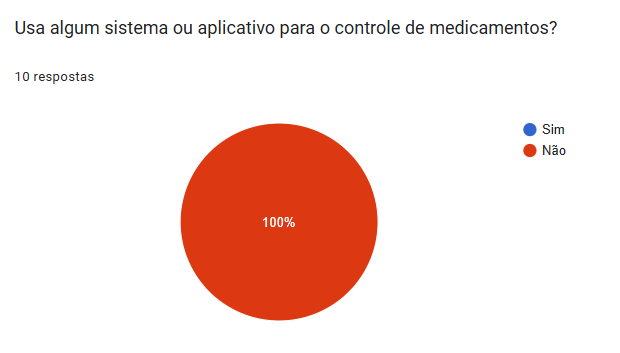
\includegraphics[width=0.75\linewidth]{assets/figuras/utiliza-app.png}
    \caption{Pergunta 6/10 do 2º Questionário}
    \fonte{Autores.}
    \label{utiliza_app}
\end{figure}

\begin{figure}[!htbp]
    \centering
    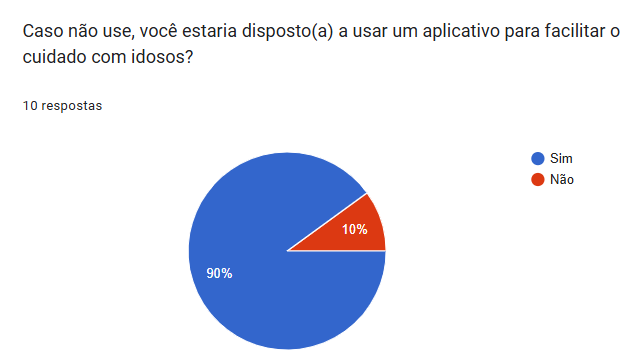
\includegraphics[width=0.75\linewidth]{assets/figuras/utilizaria-app.png}
    \caption{Pergunta 9/10 do 2º Questionário}
    \fonte{Autores.}
    \label{utilizaria_app}
\end{figure}

\break

Como apresentado nas Figuras 1 e 2, respectivamente, há uma lacuna quando se trata da rotina de controle de medicamentos de seus pacientes, mas ao mesmo tempo, há um interesse em fazer uma conversão para um sistema que atenda melhor essas necessidades. Os resultados obtidos indicam essa vontade dos profissionais em incorporar a tecnologia em suas atividades diárias.

\subsection{Ferramentas e Tecnologias}

Para a organização e acompanhamento do desenvolvimento, foi adotada uma abordagem baseada no framework Scrum, adaptada à realidade e às necessidades da equipe. O processo foi estruturado em sprints com duração de quatro semanas, com reuniões semanais para alinhamento das tarefas e revisão do progresso. As tarefas foram gerenciadas no Jira, permitindo o acompanhamento visual do fluxo de trabalho e facilitando a priorização das entregas. Essa adaptação do Scrum proporcionou maior autonomia à equipe, mantendo a organização e o foco nos objetivos do projeto.

Durante o desenvolvimento do \nomeprojeto, foram selecionadas tecnologias e ferramentas que garantem escalabilidade e facilidade de manutenção. No back-end, utilizou-se o MySQL como Sistema Gerenciador de Banco de Dados (SGBD) devido à sua confiabilidade, aliado ao framework Spring Boot em Java, que facilita a criação de APIs RESTful e a integração com outros serviços.

No front-end, optou-se pelo Angular 19, que permite o desenvolvimento de interfaces dinâmicas e reativas através de componentes. A biblioteca de componentes PrimeNG e a linguagem de design Material Design 3 foram incorporados para padronizar o design da aplicação. Para autenticação e autorização, foi utilizado o Auth0, que oferece uma solução segura e prática de Single Sign On (SSO).

Durante o desenvolvimento, o Visual Studio Code (VSCode) foi escolhido como editor de código por sua leveza, extensibilidade e integração com diversas ferramentas. O controle de versão foi realizado com o Git, utilizando o GitHub para hospedagem dos repositórios e o GitKraken para facilitar a gestão de branches e colaboração entre os membros da equipe.

A gestão de tarefas e acompanhamento do progresso do projeto foi feita com o Jira, permitindo organização eficiente das entregas e reuniões. Por fim, o Google Workspace foi utilizado para armazenamento e compartilhamento de documentos, além de servir como plataforma para aplicação dos formulários de pesquisa, através das aplicações Google Drive, Google Docs, Google Forms e Google Sheets.
	
\subsection{Processo de Desenvolvimento}

O desenvolvimento foi iniciado a partir do lado do servidor, criando o banco de dados utilizando PostgreSQL, e hospedando-o na Google Cloud Platform. O desenvolvimento do back-end e integração com banco de dados foi desenvolvida com Java e Spring Boot, e hospedada na plataforma Render.

Para o desenvolvimento do front-end, utilizou-se Angular 19 para a criação de páginas reativas, que mudam de estado. A biblioteca PrimeNG é usada para facilitar a criação de estilos dos elementos e simplificar a componentização e redução do código. Para a hospedagem, foi escolhida a plataforma Firebase.

Recursos externos foram utilizados para coleta de dados, a API "api-medicamentos-anvisa" hospedada publicamente, oferece nomes e informações úteis de todos os medicamentos registrados no Brasil até 2020. Além dela, a API de busca do Google foi utilizada por meio da ferramenta "SerperDev", da qual oferece uma interface simples à pesquisa de locais e produtos farmacêuticos.

\subsection{Equipe}

O desenvolvimento do \nomeprojeto\ se deu pela estruturação do projeto em equipe, após isso houve a designação de responsabilidades para cada colaborador. Esta seção diz sobre a organização de forma ampla e a alocação de tarefas.

O \autoref{quadro_integrantes} discorre a respeito da distribuição de tarefas da equipe. Para cada segmento do projeto foram designados ao mínimo duas pessoas, a fim de obter uma visão mais ampla de desenvolvimento; com exceção da execução de testes, que por sua natureza exige menos atenção. 

\pagebreak

\begin{quadro}[!htbp]
    \caption{\label{quadro_integrantes}Integrantes da equipe}
        \begin{tabular}{|c|c|c|c|c|c|c|}
        \hline
            Papéis & Arthur & Fernando & Henriquy & Isabella & Lucas & Mateus \\ \hline
            Back-end & & & & & \checkmark & \checkmark \\ \hline
            Front-end & \checkmark & \checkmark & & \checkmark & & \\ \hline
            Banco de Dados & & & \checkmark & & \checkmark & \\ \hline
	        Testes & & & \checkmark & \checkmark & & \\ \hline
            Documentação & \checkmark & \checkmark & \checkmark & \checkmark & \checkmark & \checkmark \\ \hline
            Design & & & \checkmark & \checkmark & & \\ \hline
            Gestão & & & \checkmark & & \checkmark & \\ \hline
        \end{tabular}
    \fonte{Autores.}
\end{quadro}

\section{Desenvolvimento}

Esta seção percorre todas as etapas do desenvolvimento do projeto, desde sua projeção de requisitos de funcionamento e regras de negócio, modelagem e prototipagem e testes.

\subsection{Requisitos}

Os requisitos do sistema, divididos em funcionais e não funcionais, detalham os recursos e as características planejadas para o projeto. A definição de cada requisito foi baseada na análise das pesquisas realizadas com o público-alvo e na avaliação da viabilidade de desenvolvimento.

\subsubsection{Requisitos Funcionais}

Requisitos funcionais são especificações que descrevem as funcionalidades e comportamentos que um sistema deve possuir para atender às necessidades dos usuários, definindo o que o sistema deve fazer e detalhando as interações entre o usuário e o software.

O requisito funcional RF04 (Notificações), criado para garantir que os usuários sejam alertados sobre eventos importantes, como horários de medicação ou consultas agendadas, o requisito funcional RF07 (Relatórios), criado para garantir que os usuários possam acompanhar a evolução clínica de pacientes por meio de relatórios detalhados e o requisito funcional RF10 (Log), incluído para registrar logs de acesso e operações críticas, como edições ou exclusões, são requisitos essenciais para garantir que o sistema atenda aos objetivos propostos e forneça valor ao público-alvo. 

Esses três itens surgiram a partir da síntese das pesquisas tanto com o público geral quanto com o público alvo da aplicação, identificando dores dos usuários e como o sistema pode ajudá-los a solucionar esses problemas. O \autoref{requisitos_f} mostra todos os requisitos funcionais criados para o \nomeprojeto.

\subsubsection{Requisitos Não-Funcionais}

Requisitos não-funcionais são especificações que descrevem as características e restrições de qualidade que o sistema deve atender para garantir sua eficiência, segurança e usabilidade. Esses requisitos não estão diretamente relacionados às funcionalidades do sistema, mas são essenciais para que ele opere de forma confiável e atenda às expectativas dos usuários.

O requisito não-funcional RNF01 (Segurança), criado para assegurar a criptografia de dados sensíveis, como senhas e informações médicas, é essencial para proteger a privacidade dos usuários e garantir conformidade com regulamentações como a LGPD. O requisito RNF06 (Desempenho), que define que o sistema deve responder às requisições em até, no máximo, 1,5 segundos, foi incluído para garantir uma experiência fluida e eficiente, especialmente em operações críticas. Já o requisito RNF10 (Disponibilidade), que exige que o sistema permaneça disponível pelo menos 99,5\% do tempo durante o horário de operação, é fundamental para assegurar que os usuários possam acessar o sistema sempre que necessário, minimizando interrupções.

Esses três requisitos foram definidos com base nas melhores práticas de desenvolvimento de software, como padrões para APIs RESTful, e nas necessidades identificadas durante a análise do público-alvo junto a reflexão sobre os requisitos funcionais. O \autoref{requisitos_nf} apresenta todos os requisitos não-funcionais criados para o sistema.

\subsection{Regras de Negócio}

Regras de negócio são diretrizes que definem como o sistema deve operar em situações específicas, garantindo que os processos sigam padrões estabelecidos. Elas são fundamentais para assegurar que o sistema funcione de maneira consistente e em conformidade com as regulamentações aplicáveis.

A regra de negócio RN02 (Segurança), que determina o arquivamento de registros excluídos por 15 dias antes da remoção definitiva, foi incluída para atender às exigências da LGPD, inclusive para permitir que os usuários tenham tempo para reverter os pedidos de exclusão ou recuperar alguma informação. A regra RN04 (Tratamentos), que exige que a conclusão ou o cancelamento de tratamentos seja realizado apenas por cuidadores autorizados e registrado em log, foi definida para garantir rastreabilidade e controle sobre ações sensíveis no sistema. Já a regra RN07 (Segurança) foi adicionada para garantir que todas informações pertencentes a um usuário devem ser armazenadas de forma segura e criptografada, a fim de respeitar normas de segurança.

Essas regras foram elaboradas com base nas necessidades do público alvo e nas regulamentações aplicáveis, como a LGPD, para garantir que o sistema seja seguro e confiável. O \autoref{regras_negocio} apresenta todas as regras de negócio definidas para a aplicação.

\subsection{Modelagem}

A modelagem do sistema é uma etapa fundamental que visa traduzir os requisitos e regras de negócio em uma representação estruturada do software. Este processo envolve os casos de uso, a definição da arquitetura, e a estrutura de dados da aplicação. Para o \nomeprojeto, a modelagem foi detalhada por meio de diagramas s de uso, que descrevem as interações entre os usuários e o sistema, o diagrama de arquitetura de sistema, que descreve como o sistema está estuturado tecnicamente e pelo modelo de entidade e relacionamento, que detalha a estrutura do banco de dados.

\subsubsection{Casos de Uso}

Como apresentado na \autoref{casos_de_uso}, os casos de uso representam as principais interações entre os usuários e o sistema, descrevendo como as funcionalidades foram projetadas para atender às necessidades identificadas durante a análise de requisitos. Eles são fundamentais para garantir que o sistema seja desenvolvido de forma alinhada às expectativas do público-alvo e às regras de negócio definidas.

\begin{figure}[!htbp]
    \centering
    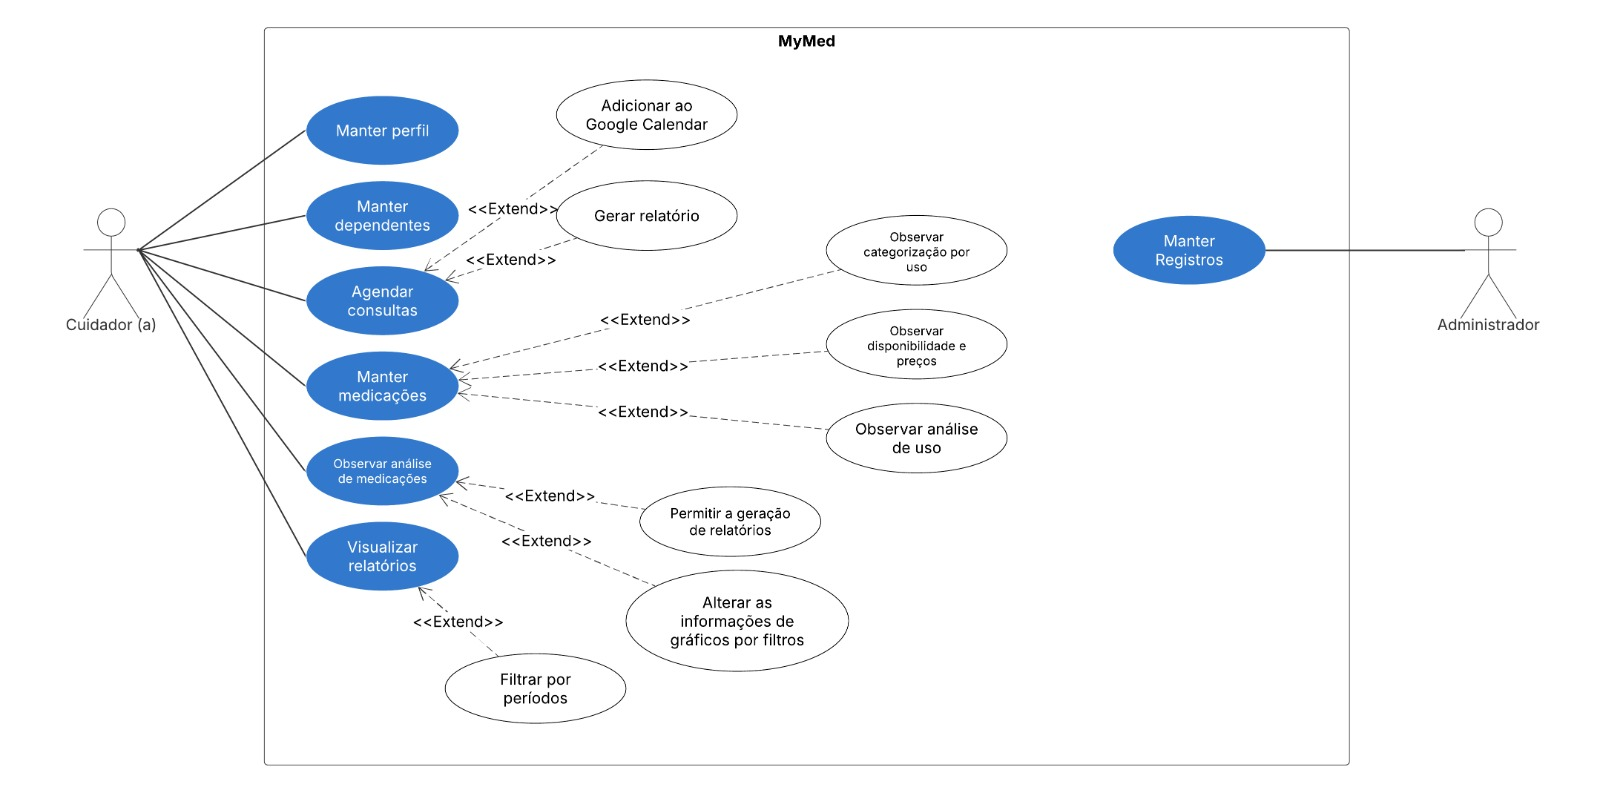
\includegraphics[width=1.0\linewidth]{assets/figuras/diagrama-casos-uso.jpg}
    \caption{Diagrama de Casos de Uso}
    \fonte{Autores.}
    \label{casos_de_uso}
\end{figure}


No \nomeprojeto, os casos de uso foram elaborados para cobrir as principais operações realizadas pelos cuidadores e administradores. Entre os casos de uso mais relevantes, destacam-se o caso de uso "Manter Dependentes" permite que o cuidador adicione, visualize, edite e exclua informações dos pacientes, garantindo que os dados estejam sempre atualizados. Já o caso de uso "Agendar Consulta" possibilita que o cuidador registre compromissos médicos em uma agenda para os pacientes, com integração opcional ao calendário do dispositivo. Além disso, o caso de uso "Gerenciar Medicações" permite o acompanhamento do estoque de medicamentos e o registro de consumo, emitindo alertas em caso de baixa disponibilidade.

O \autoref{dicionario_casos_uso} apresenta o \textit{Dicionário de Casos de Uso}, apresentando cada cenário com detalhes e informações sobre os atores envolvidos, pré-condições, fluxos principais e pós-condições.


\subsubsection{Modelo Entidade Relacionamento}

O MER do MyMed foi projetado para representar as principais entidades do sistema, como Usuário, Dependente, Consulta, Tratamento e Medicação, além de suas relações. Ele garante que as informações sejam armazenadas de forma consistente e que as interações entre as entidades sejam bem definidas. A \autoref{model_entidade_relacionamento} apresenta o diagrama completo, detalhando as entidades e seus relacionamentos.

\begin{figure}[!htbp]
    \centering
    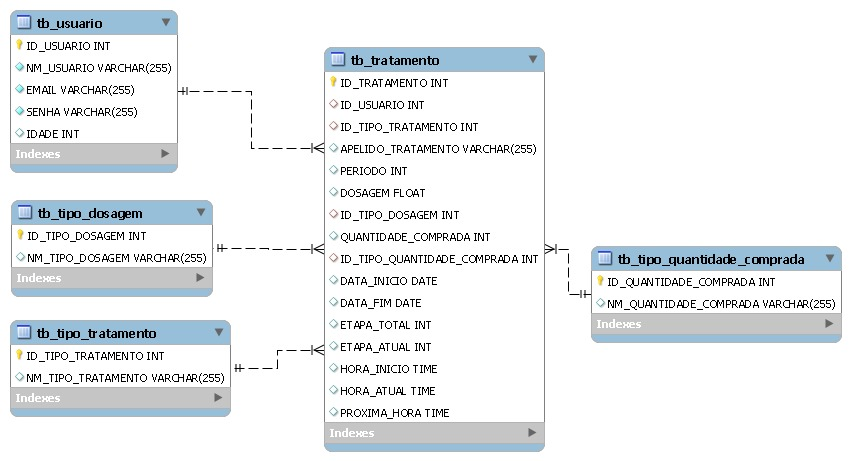
\includegraphics[width=1.0\linewidth]{assets/figuras/bancoDados.jpg}
    \caption{Imagem do Modelo Entidade Relacionamento}
    \fonte{Autores.}
    \label{model_entidade_relacionamento}
\end{figure}

Por exemplo, a entidade Usuário está relacionada à entidade Dependente, permitindo que cuidadores gerenciem os dados de seus dependentes. A entidade Consulta está associada tanto ao Usuário quanto ao Dependente, possibilitando o registro de compromissos médicos para ambos. Já a entidade Tratamento está vinculada a Medicação, permitindo o acompanhamento detalhado de medicamentos prescritos e consumidos.

O MER reflete a necessidade de um sistema robusto e escalável, garantindo que os dados sejam organizados de forma eficiente e que as operações, como consultas e atualizações, sejam realizadas de maneira confiável. Ele também assegura a integridade referencial, evitando inconsistências nos dados e permitindo que o sistema atenda aos requisitos funcionais e não funcionais definidos.

\subsection{Arquitetura de Software}

Esta subseção apresenta a arquitetura geral do sistema, suas tecnologias, infraestrutura de hospedagem e os fluxos de interação entre os contêineres. O modelo utilizado é baseado no \textit{Diagrama de Contêineres do C4 Model}.

\subsubsection{Visão Geral}

A arquitetura do sistema é composta por quatro contêineres principais, cada um com responsabilidades específicas e hospedado em diferentes plataformas de nuvem. Essa estrutura foi definida visando escalabilidade, isolamento de responsabilidades e maior confiabilidade.

A comunicação entre esses contêineres ocorre predominantemente por meio de requisições HTTP.

\begin{figure}[!htbp]
    \centering
    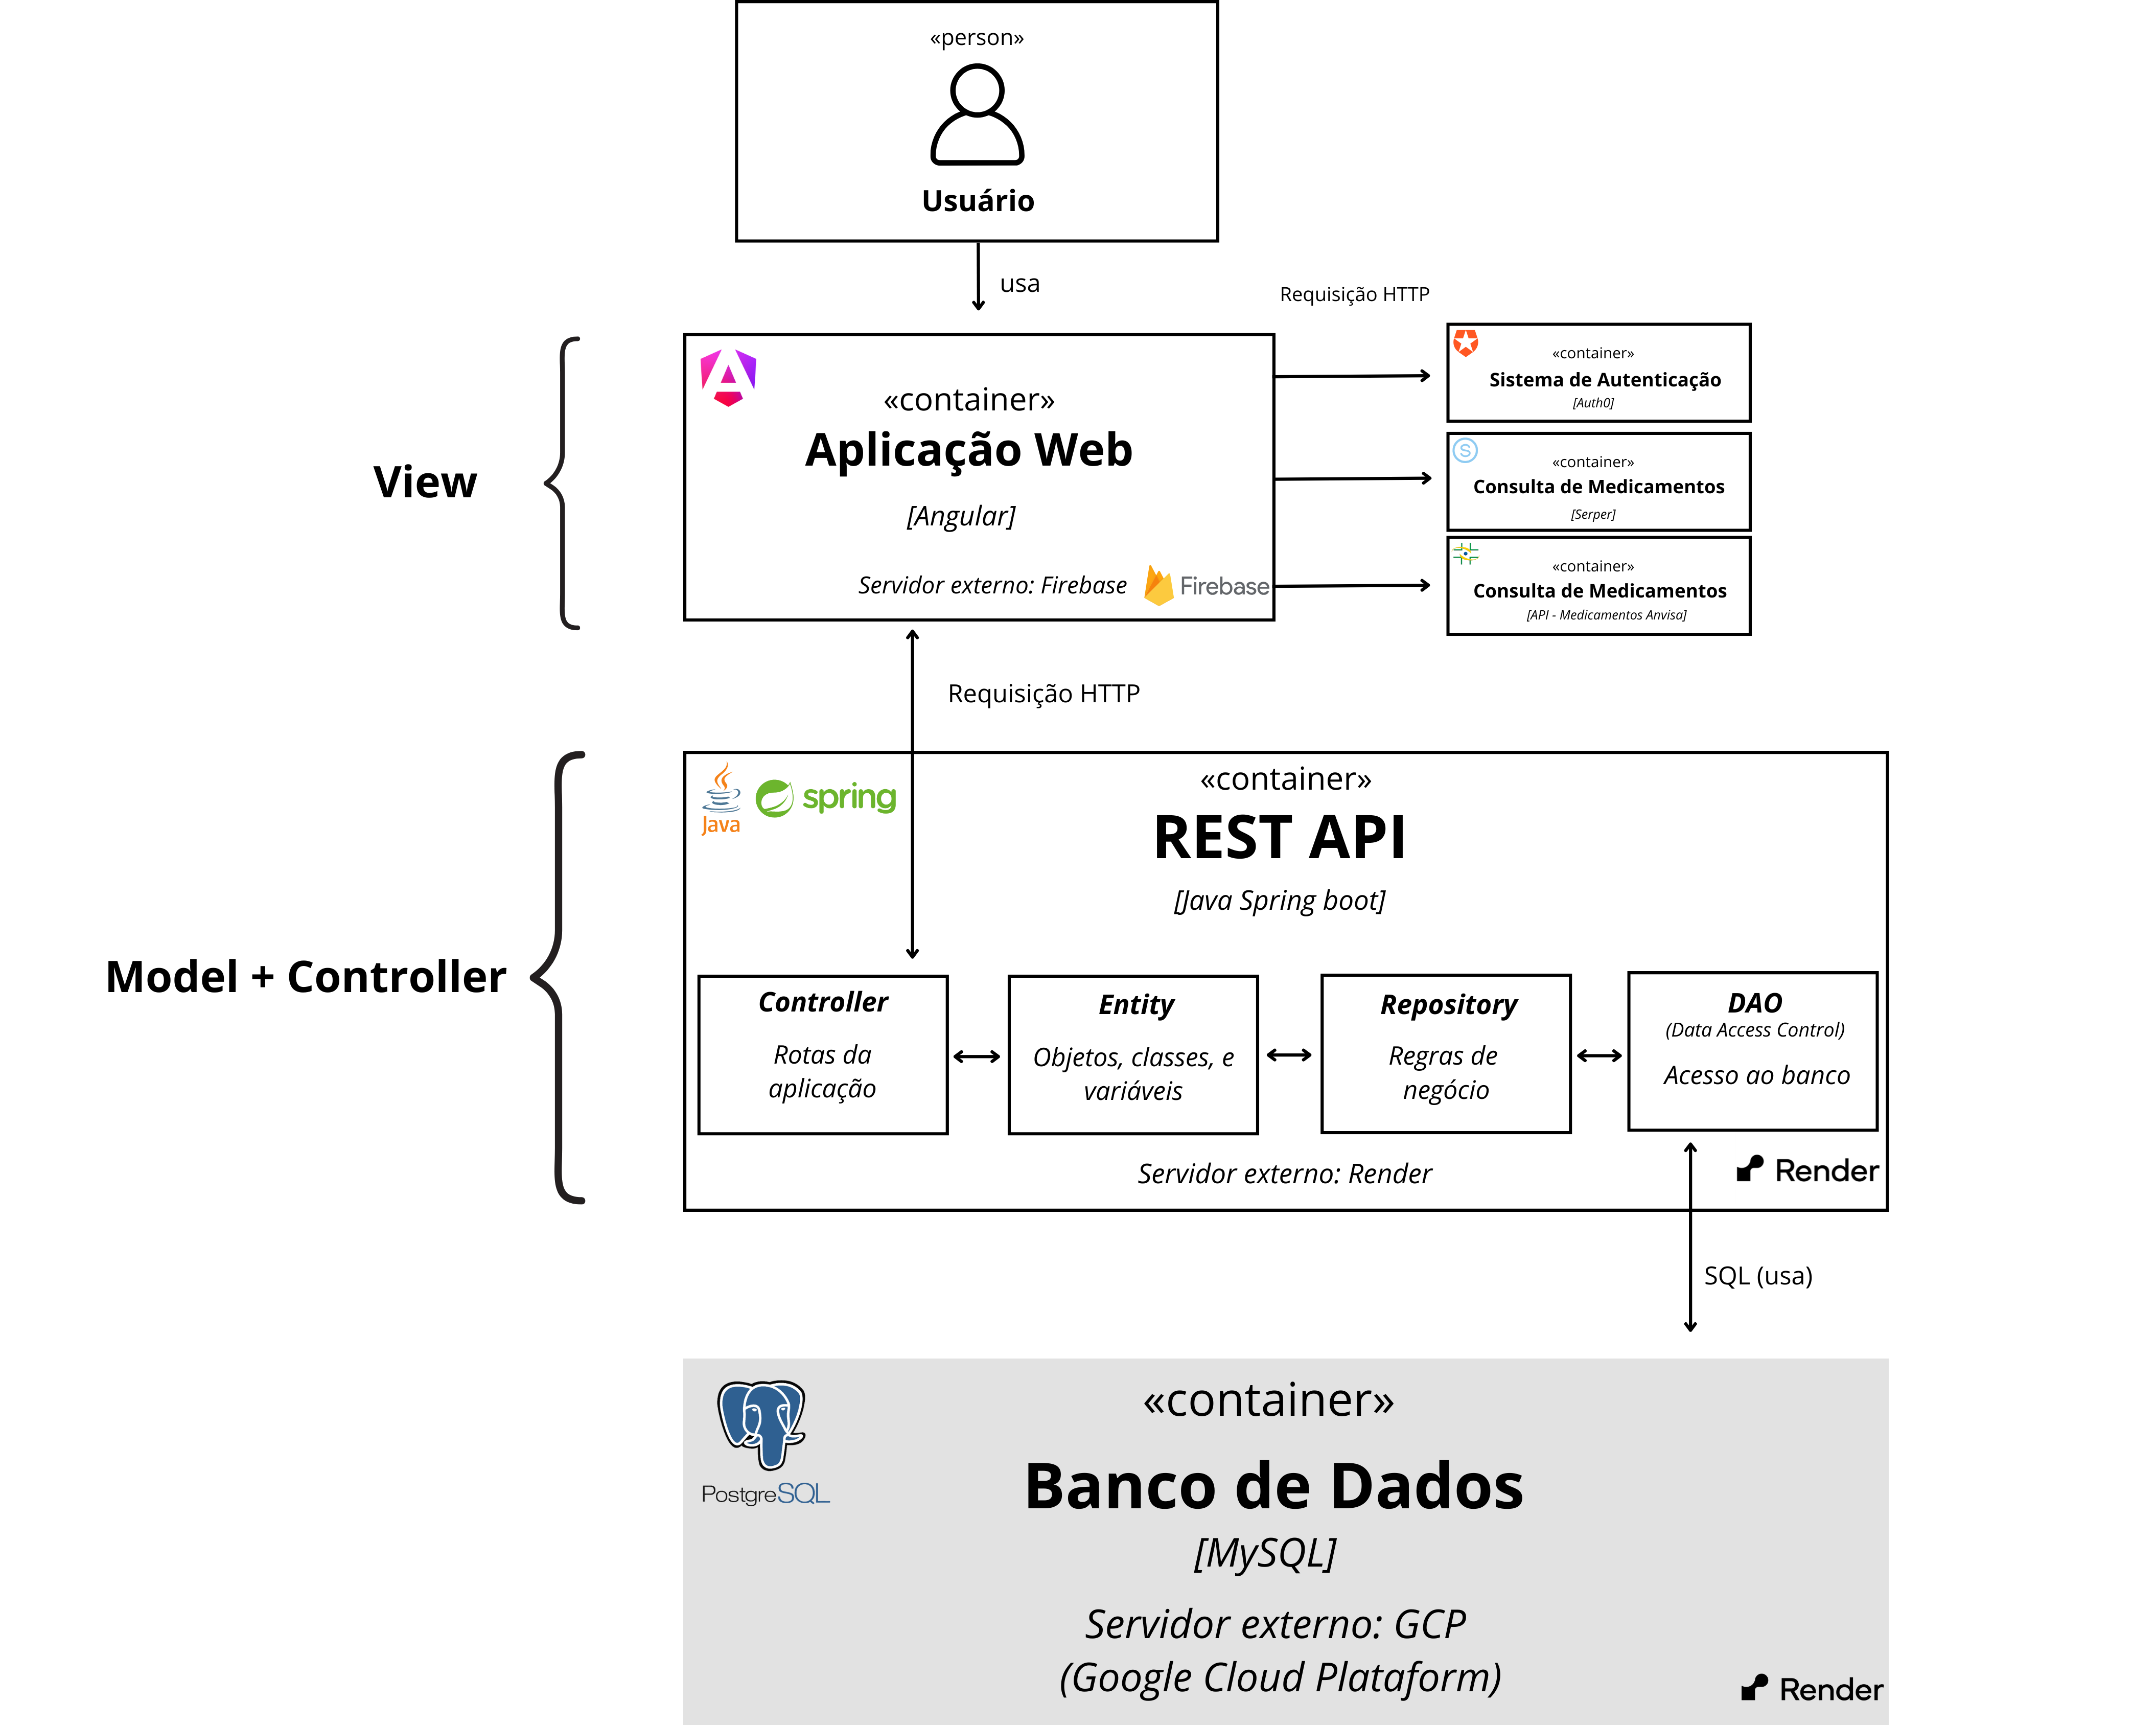
\includegraphics[width=1\textwidth]{assets/figuras/diagrama_de_software.png}
    \caption{Diagrama de Arquitetura de Software}
    \label{fig:diagrama_software}
    \fonte{Autores.}
\end{figure}

\newpage

\subsection{Prototipagem}

A prototipagem do sistema se deu pela criação inicial do conceito do sistema e fluxos de dados com baixo nível de detalhamento. Depois que aprovado, houve a criação de protótipos de alta fidelidade na plataforma \textit{Figma}. O apêndice \autoref{prototipagem} nos traz mais detalhes sobre as telas do sistema, como a tela inicial, calendário, gráficos, perfil de usuário, entre as outras criadas para montar um fluxo completo e adequado.

\renewcommand{\arraystretch}{1.5} % 1.5 = 50% mais alto que o normal

\subsection{Plano de Testes}

O plano de testes visa verificar todas as funcionalidades e validar seu uso na aplicação. O \autoref{plano_testes} retrata com detalhes e maior descrição todos os testes que devem ser implementados nos diversos segmentos do sitema, como a verificação da conexão com o banco de dados, validação de informações de usuário e exibição correta de consultas conforme a data do dispositivo.

\subsection{Criptografia}

Para garantir a segurança na comunicação entre os usuários e a aplicação, foi configurado o protocolo HTTPS com suporte a TLS, utilizando certificados digitais válidos e atualizados. A certificação foi realizada através da integração com o serviço Let's Encrypt através do Render para o back-end e Gerenciado pelo Google para o front-end através do Firebase Hosting, assegurando criptografia ponta a ponta durante as transações de dados. A configuração foi validada na ferramenta SSL Labs, onde o ambiente obteve a nota máxima A+.

\begin{figure}[h!]
    \centering
    \begin{subfigure}[b]{0.45\textwidth}
        \centering
        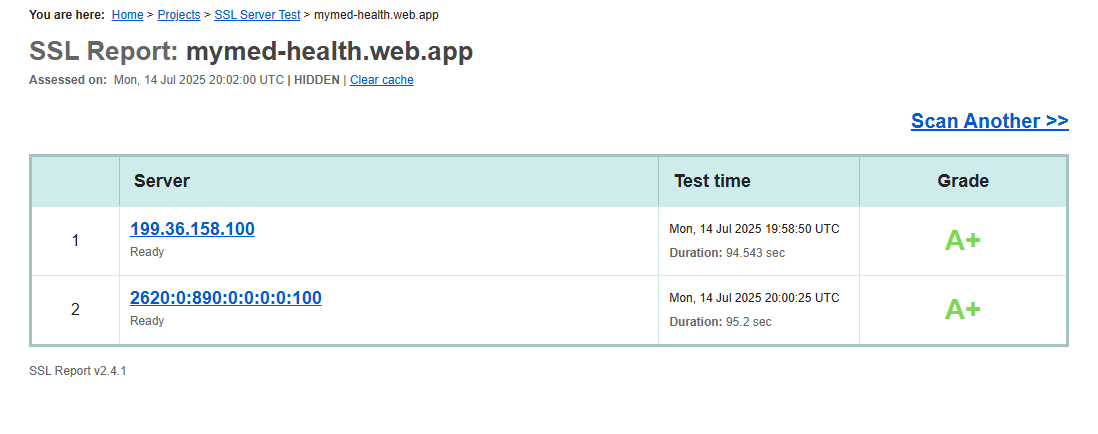
\includegraphics[width=\textwidth]{assets/figuras/certificacao_front.png}
        \caption{Resultado dos testes do front-end}
    \end{subfigure}
    \hfill
    \begin{subfigure}[b]{0.45\textwidth}
        \centering
        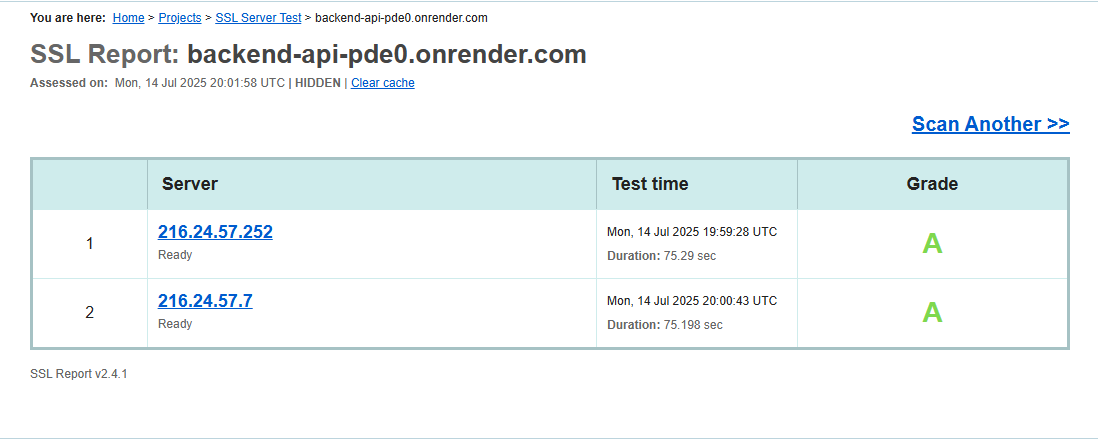
\includegraphics[width=\textwidth]{assets/figuras/certificacao_back.png}
        \caption{Resultado dos testes do back-end}
    \end{subfigure}
    \label{fig:testes-criptografia}
    \caption{Resultados dos testes de criptografia.}
    \fonte{Autores.}
\end{figure}

% \section{MVP}

% "O MVP é o menor conjunto de recursos que permite que o empreendedor comece o processo de aprendizado com o mínimo de esforço e o máximo de aprendizado validado sobre os clientes."

% "Uma ferramenta para testar hipóteses de negócios e iniciar o aprendizado, coletando o máximo de informações validadas sobre os clientes com o menor esforço possível."


% ---
% Finaliza a parte no bookmark do PDF, para que se inicie o bookmark na raiz
% ---
\bookmarksetup{startatroot}% 

% ---

% ---
% Conclusão
% ---
\section{Resultado e discussões}
Esta seção apresenta os principais resultados obtidos ao longo do desenvolvimento do projeto, bem como a análise crítica desses achados. São expostos os avanços alcançados, as limitações identificadas e os impactos observados no desempenho e na usabilidade do sistema. Além disso, busca-se discutir de que forma os resultados se relacionam com os objetivos propostos inicialmente, destacando pontos fortes, fragilidades e oportunidades de melhoria para trabalhos futuros.

\subsection {Problemas no desenvolvimento}
Durante o desenvolvimento do projeto, surgiram problemas que afetaram tanto o cronograma quanto a implementação de algumas funcionalidades. No início, a escassez de pesquisas e documentações dificultou o embasamento do projeto. Além disso, a necessidade frequente de corrigir bugs consumiu mais tempo do que o previsto, atrasando etapas importantes do desenvolvimento.

No âmbito técnico, enfrentamos desafios relacionados à compatibilidade de versões e bibliotecas, integração entre módulos e limitações de ferramentas, como o banco de dados. Este último precisou ser migrado para uma instância diferente devido às restrições da plataforma GCP, exigindo ajustes adicionais, como a renovação da instância a cada 30 dias e a reexecução das migrations.

Na camada de segurança, inicialmente o front-end não garantia a criptografia de todas as requisições HTTP, resultando em transmissão de dados em texto claro, o que poderia expor o sistema a ataques como SQL injection ou vazamento de informações sensíveis. Além disso, o mecanismo de autenticação era básico, sem suporte robusto para autorização. A solução envolveu configurar adequadamente o HTTPS/TLS para todas as comunicações e implementar um sistema de autenticação baseado em JWT (JSON Web Token), protegendo as requisições contra acessos não autorizados.

Por fim, embora os esforços de otimização tenham melhorado o desempenho, não foi possível atingir a latência média de 1,5 segundos definida como requisito não-funcional. Ainda assim, os resultados foram satisfatórios para a maioria das operações e atenderam aos limites do projeto.

Esses desafios, embora complexos, proporcionaram aprendizado significativo e contribuíram para o aprimoramento do processo de desenvolvimento, garantindo a continuidade e a consolidação dos resultados.

\subsection {Resultados dos testes internos}

Os testes internos, presentes no plano de testes, cobriram as funcionalidades essenciais do sistema, desde a gestão administrativa de usuários até o acompanhamento clínico detalhado dos pacientes e a integração com serviços externos.

\subsubsection{Aspectos positivos}
Os resultados positivos demonstram a correta execução das funcionalidades primárias do sistema. Em um cenário de sucesso, todas as operações de CRUD (Criação, Edição e Exclusão) para usuários, administradores, pacientes, consultas e informações adicionais de perfil são persistidas com sucesso no banco de dados, confirmando a eficácia da lógica de negócios e da query SQL. Além disso, a adição de medicamentos a um tratamento e a manutenção dos registros cardiovasculares e glicêmicos foram concluídas, indicando que os dados brutos de saúde são armazenados corretamente.

A integração com serviços externos também apresentou sucesso: o sistema foi capaz de pesquisar e visualizar farmácias e medicamentos a venda ao se conectar com sucesso às APIs externas, confirmando a funcionalidade adequada dos mecanismos de comunicação e autenticação. Por fim, a visualização correta de consultas por filtro de data e a exibição dos gráficos de adesão e intercorrências indicam que a recuperação e apresentação de dados funcionam conforme o esperado.

\subsubsection{Aspectos negativos}

Um erro que aconteceu em alguns cenários foi que, mesmo sem todos os campos obrigatórios preenchidos, ainda ocorria qualquer tipo de persistência de dados. Este é um risco de infraestrutura que pode invalidar algumas operações do back-end, e além disso, quebrava a renderização de algumas informações em diversas telas da aplicação.

O teste de notificação demonstrava alguns erros mais graves em termos de integridade de dados e experiência do usuário: a notificação não aparecia ou poderia aparecer no horário errado.

Por fim, a integração externa depende da disponibilidade da API e da ativação de funcionalidades no dispositivo do usuário, como o GPS estar desligado, que impede a pesquisa por proximidade mesmo que a API funcione perfeitamente.

\subsection {Resultados dos testes externos}

\subsubsection{Aspectos positivos}

Os resultados positivos confirmam a solidez do back-end do sistema em suas operações fundamentais. Em condições ideais de rede e conectividade, as operações de CRUD relacionadas aos usuários, pacientes e consultas foram concluídas com sucesso. Isso valida a lógica de negócios e a integridade das transações sob uma variedade de dispositivos e outros ambientes. A capacidade de adicionar medicamentos a um tratamento e registro de dados contínuos de saúde, como pressão arterial e nível de glicose, também deram certo. A integração com as APIs externas demonstrou ser robusta, conseguindo permitir a pesquisa de farmáciase a visualização de medicamentos de forma rápida e precisa para a maioria dos testadores.

\subsubsection{Aspectos negativos}
Alguns problemas foram identificados no processo de testes externos foram que o login não é validado corretamente no backend, comprometendo a segurança do sistema. Além disso, não foi possível abrir a foto do paciente no backend, o que limita a visualização de informações relevantes. Outro fator crítico está relacionado ao tempo de inicialização da API, que pode levar alguns segundos até ficar ativa, impedindo o acesso imediato à aplicação. Soma-se a isso a ausência de implementação das claims/roles, permitindo que em alguns cenários, usuários realizem requisições sem restrições, o que representa um risco de uso indevido.

\subsection{Empresa}
Na disciplina de Gestão Industrial (GEI), como atividade avaliativa do segundo bimestre, desenvolveu-se a estrutura empresarial fictícia da equipe Hyperion, cujo produto principal é o \nomeprojeto. O projeto apresenta a identidade da empresa, análise de mercado, modelo de negócio, estratégias de marketing e outros, e foi importante para que desenvolvessemos uma visão mais ampliada e descritiva do que o \nomeprojeto e a Equipe Hyperion significa para pessoas de fora das matérias técnicas, possibilitando para que elas pudessem entender também. Todos os detalhes sobre a empresa pode ser consultada no \autoref{secao_empresa}.

\section{Conclusão}
O desenvolvimento do MyMed demonstrou a importância da tecnologia como ferramenta de apoio à saúde e ao cuidado de idosos, especialmente em um contexto onde a demanda por serviços de cuidado segue em crescimento constante, fator identificado durante meses de pesquisas e estudos, incluindo análises das necessidades dos cuidadores e implementações de funcionalidades que pudessem beneficiar inclusive os dependentes, mesmo que de forma indireta.

De forma técnica, um dos objetivos do projeto foi a criação de uma API eficiente e bem documentada, que possa facilitar e possibilitar a integração e o uso por terceiros. Para suportar essa arquitetura de maior escala, houve a criação de uma estrutura robusta para o front-end também, com enfoque em conseguir proporcionar uma navegação intuitiva e uma boa experiência para os usuários. No entanto, desafios relacionados à segurança, desempenho e estabilidade da aplicação foram identificados nesse processo, indicando áreas que necessitam de correções e melhorias contínuas para alcance de um público maior. Mesmo diante de limitações técnicas, esses resultados evidenciam que o projeto alcançou, em grande parte, os objetivos de promover acessibilidade e usabilidade para o público-alvo.

Por fim, este trabalho demonstra que o investimento em tecnologia aplicada à saúde e ao cuidado de idosos contribui com a melhoria de rotina de cuidados e com a promoção de autonomia, segurança e qualidade de vida. Os resultados obtidos evidenciam que, mesmo diante de limitações técnicas, é possível desenvolver sistemas relevantes e funcionais, que podem servir de referência para projetos futuros. Desta forma, o MyMed não apenas cumpre sua função prática, mas também reforça a importância de soluções inovadoras e adaptáveis entre tecnologia e cuidado / saúde humana.

\postextual



\newpage

\bibliography{referencias}
% ---
% Inicia os apêndices
% ---
\newpage
\begin{apendicesenv}

% % % % ----------------------------------------------------------
\chapter{Pesquisas\label{pesquisas}}

As pesquisas foram conduzidas para entender melhor as necessidades e desafios enfrentados pelos usuários e cuidadores de idosos. A seguir, apresentamos as perguntas formuladas para cada grupo respectivo. Os formulários foram aplicados por meio don Google Forms, garantindo a coleta de dados de forma organizada e acessível.

\section{Pesquisa com o Público Geral}
\begin{enumerate}
    \item Se não se importar, poderia informar o seu nome? (a resposta não é obrigatória)
    \item Você já utilizou alguma aplicação ou sistema de auxílio no gerenciamento de medicamentos/consultas? (Sim ou Não)
    \item Se sim, se importa de compartilhar sua experiência? Como é o aplicativo? (Resposta livre)
    \item Você possui alguma dificuldade ao lidar com tratamentos com remédios? (Lembrar os horários, Dosagens, Reposição dos remédios, Nenhuma)
    \item Você possui alguma dificuldade ao lidar com vacinas? (Lembrar as datas, Disponibilidade, Nenhuma)
    \item Você possui alguma dificuldade ao lidar com consultas? (Lembrar a data e/ou horário de agendamento, Organização, Nenhuma)
    \item No momento atual, o que você considera sua maior dificuldade ao gerenciar seus tratamentos e/ou compromissos médicos? (Resposta livre)
    \item Já utilizou algum serviço de Teleconsulta? (Sim ou Não)
    \item Se sim, se importa de compartilhar sua experiência? Foi positiva ou negativa? (Resposta livre)
    \item Já utilizou algum serviço de Tele-educação voltado à área da saúde? (Sim ou Não)
    \item Se sim, se importa de compartilhar sua experiência? Foi positiva ou negativa? (Resposta livre)
    \item Consegue dizer um processo, que se fosse automático, auxiliaria você no gerenciamento de seus compromissos médicos nos dias atuais? Se sim qual? (Resposta livre)
\end{enumerate}

\section{Pesquisa com Cuidadores de Idosos}
\begin{enumerate}
    \item Qual sua função atual? (Cuidador(a), Coordenador(a), Enfermeiro(a), Outros)
    \item Você trabalha em: (Asilo, Casa de repouso, Domicílio particular, Outros)
    \item Quantos idosos você(s) cuida(m) atualmente? (1-5, 5-20, 20-50, 50+)
    \item Quais atividades fazem parte da sua rotina com os idosos? [Marque todas que se aplicam] (Administração de medicamentos, Monitoramento de sinais vitais, Acompanhamento em consulta, Outros)
    \item Como você organiza os horários e dosagens dos medicamentos dos idosos? (Resposta livre)
    \item Usa algum sistema ou aplicativo para o controle de medicamentos? (Sim ou Não)
    \item Se sim, qual? (Resposta livre)
    \item Como você registra a rotina e as informações de saúde dos idosos? [Marque todas que se aplicam] (Aplicativos ou softwares, Papel, Planilhas (Excel, Google Sheets), Não Registro)
    \item Caso não use, você estaria disposto(a) a usar um aplicativo para facilitar o cuidado com idosos? (Sim ou Não)
    \item O que esse app deveria ter para ser útil no seu dia a dia? (Resposta livre)
\end{enumerate}


\newpage

\chapter{Requisitos Funcionais\label{requisitos_f}}

Os requisitos funcionais do sistema são apresentados a seguir, servindo de descrição das principais funcionalidades que o sistema deve oferecer.

\renewcommand{\arraystretch}{1.5} % 1.5 = 50% mais alto que o normal

\begin{quadro}
    \caption{\label{quadro_requisitos_f}Requisitos Funcionais}
    \begin{tabular}{|c|c|p{10cm}|}
        \hline
        \textbf{Código} & \textbf{Categoria} & \textbf{Descrição} \\ \hline
        RF01   & Cadastro     & Cadastrar paciente: dados pessoais (nome, CPF, data de nascimento, endereço, contato, etc.) \\ \hline
        RF02   & Paciente     & Visualizar perfil do paciente: histórico de atendimentos e tratamentos \\ \hline
        RF03   & Paciente     & Editar e atualizar dados do paciente \\ \hline
        RF04   & Cadastro     & Excluir cadastro de paciente: mas mantendo o histórico arquivado \\ \hline
        RF05   & Consulta     & Agendar nova consulta: paciente, profissional, data, hora e local \\ \hline
        RF06   & Consulta     & Listar consultas agendadas: com filtros por data, profissional ou paciente \\ \hline
        RF07   & Consulta     & Editar ou cancelar consulta: antes da data marcada \\ \hline
        RF08   & Atendimento  & Registrar atendimento: diagnóstico, conduta, recomendações, etc. \\ \hline
        RF09   & Notificação  & Emitir alertas ou notificações: consultas futuras \\ \hline
        RF10   & Tratamento   & Criar plano de tratamento: associado a um paciente e diagnóstico \\ \hline
        RF11   & Tratamento   & Listar tratamentos em andamento, concluídos ou cancelados (tipo kanban) \\ \hline
        RF12   & Tratamento   & Registrar evolução do tratamento: observações por etapa ou sessão \\ \hline
        RF13   & Tratamento   & Anexar prescrições médicas: laudos, imagens ou documentos ao tratamento \\ \hline
        RF14   & Relatório    & Gerar relatórios de acompanhamento: paciente, profissional ou período \\ \hline
        RF15   & Histórico    & Visualizar histórico de consultas: evolução clínica \\ \hline
        RF16   & Exportação   & Exportar dados: PDF, Excel ou outro formato \\ \hline
        RF17   & Autenticação & Autenticar usuários: login e senha \\ \hline
        RF18   & Permissão    & Gerenciar permissões: admin, profissional de saúde, recepcionista, etc. \\ \hline
        RF19   & Log          & Registrar logs de acesso: operações críticas (como edições e exclusões) \\ \hline
        RF20   & Pesquisa     & Pesquisar pacientes, consultas e tratamentos: múltiplos critérios \\ \hline
        RF21   & Filtro       & Aplicar filtros e ordenações nas pesquisas \\ \hline
    \end{tabular}
    \fonte{Autores.}
\end{quadro}


\newpage

\chapter{Requisitos Não Funcionais\label{requisitos_nf}}

Os requisitos não funcionais do sistema são apresentados a seguir, servindo de descrição das principais características que o sistema deve atender.

\renewcommand{\arraystretch}{1.5} % 1.5 = 50% mais alto que o normal

\begin{quadro}
    \caption{\label{quadro_requisitos_nf}Requisitos Não Funcionais}
    \begin{tabular}{|c|c|p{10cm}|}
        \hline
        \textbf{Código} & \textbf{Categoria} & \textbf{Descrição} \\ \hline
        RNF01  & Segurança       & Criptografia de dados sensíveis: como senhas e informações médicas \\ \hline
        RNF02  & Acesso          & Controle de acesso baseado em perfis de usuário: admin ou cuidador \\ \hline
        RNF03  & Sessão          & Validação de sessão com expiração automática por inatividade \\ \hline
        RNF04  & Backup          & Backups regulares e automáticos: para recuperação de dados \\ \hline
        RNF05  & Desempenho      & O sistema deve responder às requisições em até 5 segundos nas operações \\ \hline
        RNF06  & Concorrência    & Suportar múltiplos acessos simultâneos sem perda de desempenho \\ \hline
        RNF07  & Interface       & Interface intuitiva e acessível para usuários não técnicos \\ \hline
        RNF08  & Design          & Uso de padrões de design consistentes e amigáveis \\ \hline
        RNF09  & Manutenção      & O código-fonte deve ser modular e documentado, facilitando a manutenção \\ \hline
        RNF10  & Arquitetura     & Uso de arquitetura escalável \\ \hline
        RNF11  & Disponibilidade & O sistema deve estar disponível pelo menos 99,5\% do tempo \\ \hline
        RNF12  & Integridade     & Deve garantir integridade dos dados em operações simultâneas \\ \hline
        RNF13  & Recuperação     & Deve ser capaz de recuperar-se de falhas sem perda de dados \\ \hline
        RNF15  & Ambientes       & Ambientes separados para produção, testes e homologação \\ \hline
        RNF16  & Segurança       & O sistema deve exigir autenticação de usuário para qualquer operação de inserção, alteração ou exclusão de dados \\ \hline
    \end{tabular}
    \fonte{Autores.}
\end{quadro}


\newpage

\chapter{Regras de Negócio\label{regras_negocio}}

As regras de negócio são fundamentais para garantir o correto funcionamento do sistema, assegurando que as operações atendam aos requisitos legais e funcionais. A seguir, apresentamos uma tabela com as principais regras de negócio definidas para o sistema de gestão de dependentes.

\renewcommand{\arraystretch}{1.5} % 1.5 = 50% mais alto que o normal

\begin{quadro}
    \caption{\label{quadro_regras_negocio}Regras de Negócio}
    \begin{tabular}{|c|c|p{10cm}|}
        \hline
        \textbf{Código} & \textbf{Categoria} & \textbf{Descrição} \\ \hline
        RN01   & Cadastro     & Apenas usuários com permissão de cuidador ou administrador podem cadastrar pacientes. \\ \hline
        RN02   & Segurança   & A exclusão de qualquer registro relacionado a um usuário, como o perfil de um paciente ou seu próprio perfil, deve arquivar todo o histórico sem remoção definitiva do banco de dados durante 15 dias, conforme prazo de resposta da LGPD. \\ \hline
        RN03   & Tratamentos & Um plano de tratamento só pode ser criado se houver, no momento do registro, ao menos um diagnóstico relacionado. \\ \hline
        RN04   & Tratamentos & A conclusão ou o cancelamento de um tratamento só podem ser realizados por cuidadores com permissão e devem ser registrados em log. \\ \hline
        RN05   & Tratamentos & A evolução de um tratamento deve ser registrada obrigatoriamente com data, cuidador responsável e observações. \\ \hline
        RN06   & Tratamentos & Prescrições médicas devem ser anexadas em formato válido (PDF, JPG, PNG, etc.), respeitando o tamanho máximo definido para cada tipo de arquivo. \\ \hline
        RN07   & Segurança   & O armazenamento de todos os dados relacionados a um usuário, incluindo backups, devem ser realizados em ambientes seguros, hospedados em servidores certificados e com criptografia válida. \\ \hline
        RN08   & Privacidade & O sistema deve solicitar consentimento explícito do usuário para a coleta e o armazenamento de dados sensíveis. \\ \hline
    \end{tabular}
    \fonte{Autores.}
\end{quadro}


\newpage

\chapter{Dicionário de Casos de Uso\label{dicionario_casos_uso}}

A seguir consta o dicionário de casos de uso do sistema, que descreve as principais funcionalidades e interações dos usuários com o sistema. Cada caso de uso é detalhado com informações sobre o ator, pré-condições, fluxo principal e pós-condição.



\begin{quadro}
    \caption{\label{quadro_manter_perfil}Manter Perfil}
    \begin{tabular}{|l|p{12cm}|}
        \hline
        \textbf{Caso de Uso} & Manter Perfil \\ \hline
        \textbf{Descrição} & Permite ao cuidador(a) visualizar e editar suas informações pessoais. \\ \hline
        \textbf{Ator} & Cuidador(a) \\ \hline
        \textbf{Pré-condições} & Estar autenticado (logado) \\ \hline
        \textbf{Fluxo Principal} & 1. Cuidador acessa a seção de configuração do perfil \newline 2. Visualiza os dados cadastrados \newline 3. Edita os registros de cuidador \\ \hline
        \textbf{Extensões} & N/A \\ \hline
        \textbf{Pós-condição} & Dados do perfil atualizado com sucesso \\ \hline
    \end{tabular}
    \fonte{Autores.}
\end{quadro}


\begin{quadro}
    \caption{\label{quadro_manter_dependentes}Manter Dependentes}
    \begin{tabular}{|l|p{12cm}|}
        \hline
        \textbf{Caso de Uso} & Manter Dependentes \\ \hline
        \textbf{Descrição} & Permite ao cuidador(a) adicionar, visualizar, editar e excluir dados de dependentes. \\ \hline
        \textbf{Ator} & Cuidador(a) \\ \hline
        \textbf{Pré-condições} & Estar autenticado (logado) \\ \hline
        \textbf{Fluxo Principal} & 1. Cuidador acessa a seção de configuração do perfil \newline 2. Visualiza os dados dos dependentes \newline 3. Edita ou remove os dados dos dependentes \\ \hline
        \textbf{Extensões} & N/A \\ \hline
        \textbf{Pós-condição} & Dados do perfil atualizado com sucesso \\ \hline
    \end{tabular}
    \fonte{Autores.}
\end{quadro}


\begin{quadro}
    \caption{\label{quadro_agendar_consulta}Agendar Consulta}
    \begin{tabular}{|l|p{12cm}|}
        \hline
        \textbf{Caso de Uso} & Agendar Consulta \\ \hline
        \textbf{Descrição} & Cuidador(a) agendar consultas para os dependentes. \\ \hline
        \textbf{Ator} & Cuidador(a) \\ \hline
        \textbf{Pré-condições} & Estar autenticado (logado) \\ \hline
        \textbf{Fluxo Principal} & 1. Cuidador acessa a funcionalidade de agendamento \newline 2. Seleciona data e horário \newline 3. Adiciona apelido \newline 4. Confirma o agendamento \\ \hline
        \textbf{Extensões} & Adicionar ao Google Calendar ou integrar ao calendário do dispositivo utilizado via arquivo .ics \textless\textless extend\textgreater\textgreater \newline Gerar relatório \textless\textless extend\textgreater\textgreater \\ \hline
        \textbf{Pós-condição} & Consulta agendada e registrada no sistema \\ \hline
    \end{tabular}
    \fonte{Autores.}
\end{quadro}


\begin{quadro}
    \caption{\label{quadro_gerenciar_medicacoes}Gerenciar Medicações do Dependente}
    \begin{tabular}{|l|p{12cm}|}
        \hline
        \textbf{Caso de Uso} & Gerenciar medicações do dependente \\ \hline
        \textbf{Descrição} & Permite ao cuidador visualizar, atualizar e acompanhar o uso dos medicamentos de um dependente, incluindo o estoque e registros de consumo. \\ \hline
        \textbf{Ator} & Cuidador(a) \\ \hline
        \textbf{Pré-condições} & Estar autenticado (logado) \\ \hline
        \textbf{Fluxo Principal} & 1. Acessar módulo de medicações \newline 2. Visualizar dados de cada medicamento \newline 3. Registrar consumo \newline 4. Atualizar estoque disponível \\ \hline
        \textbf{Extensões} & Calcular índice de adesão ao tratamento \textless\textless extend\textgreater\textgreater \newline Exibir alertas de baixo estoque \textless\textless extend\textgreater\textgreater \newline Redirecionar para busca de preços e disponibilidade \textless\textless extend\textgreater\textgreater \\ \hline
        \textbf{Pós-condição} & Dados dos medicamentos atualizados; adesão e estoque recalculados. \\ \hline
    \end{tabular}
    \fonte{Autores.}
\end{quadro}


\begin{quadro}
    \caption{\label{quadro_visualizar_analises_medicamentos}Visualizar Análises de Uso de Medicamentos}
    \begin{tabular}{|l|p{12cm}|}
        \hline
        \textbf{Caso de Uso} & Visualizar análises de uso de medicamentos \\ \hline
        \textbf{Descrição} & Exibe gráficos e indicadores sobre o uso dos medicamentos, como frequência, horários, aderência e possíveis anomalias. \\ \hline
        \textbf{Ator} & Cuidador(a) \\ \hline
        \textbf{Pré-condições} & Estar autenticado (logado) \\ \hline
        \textbf{Fluxo Principal} & 1. Acessar seção de análises de medicação \newline 2. Visualizar gráficos com dados de uso \\ \hline
        \textbf{Extensões} & N/A \\ \hline
        \textbf{Pós-condição} & Gráficos e relatórios exibidos com base nos dados registrados. \\ \hline
    \end{tabular}
    \fonte{Autores.}
\end{quadro}

\begin{quadro}
    \caption{\label{quadro_observar_analise_medicacao}Observar Análise de Medicação}
    \begin{tabular}{|l|p{12cm}|}
        \hline
        \textbf{Caso de Uso} & Observar análise de medicação \\ \hline
        \textbf{Descrição} & Permite ao cuidador(a) visualizar e gerenciar as informações associadas aos tratamentos dos dependentes, como informações gerais, categorização e análise por uso e disponibilidade através de gráficos. \\ \hline
        \textbf{Ator} & Cuidador(a) \\ \hline
        \textbf{Pré-condições} & Estar autenticado (logado) \\ \hline
        \textbf{Fluxo Principal} & 1. Cuidador acessa a seção de medicações \newline 2. Visualiza as análises e informações sobre os medicamentos. \\ \hline
        \textbf{Extensões} & Permite a geração de relatórios \textless\textless extends\textgreater\textgreater \newline Alterar as informações de gráficos através de filtros \textless\textless extends\textgreater\textgreater \\ \hline
        \textbf{Pós-condição} & Dados de um tratamento do dependente visualizados com sucesso \\ \hline
    \end{tabular}
    \fonte{Autores.}
\end{quadro}

\begin{quadro}
    \caption{\label{quadro_controlar_registros}Controlar Registros}
    \begin{tabular}{|l|p{12cm}|}
        \hline
        \textbf{Caso de Uso} & Controlar Registros \\ \hline
        \textbf{Descrição} & Permite que o administrador realize o controle de usuários e atualizações ao sistema (excluir cuidadores caso haja mau uso, corrigir erros…) \\ \hline
        \textbf{Ator} & Administrador \\ \hline
        \textbf{Pré-condições} & Acessar com credenciais de administrador \\ \hline
        \textbf{Fluxo Principal} & 1. O sistema monitora ações do cuidador. \newline 2. Registra alterações ou eventos automaticamente. \newline 3. Atualiza banco de dados conforme necessário. \\ \hline
        \textbf{Extensões} & Editar dados do cuidador \textless\textless extend\textgreater\textgreater \newline Editar dados dos dependentes \textless\textless extend\textgreater\textgreater \newline Excluir registros \textless\textless extend\textgreater\textgreater \\ \hline
        \textbf{Pós-condição} & Registros atualizados e armazenados corretamente pelo sistema. \\ \hline
    \end{tabular}
    \fonte{Autores.}
\end{quadro}


\begin{quadro}
    \caption{\label{quadro_visualizar_relatorios}Visualizar Relatórios}
    \begin{tabular}{|c|p{12cm}|}
        \hline
        \textbf{Caso de Uso} & Visualizar Relatórios \\ \hline
        \textbf{Descrição} & Permite ao cuidador(a) gerar relatórios de adesão ao tratamento e resultados de consultas. \\ \hline
        \textbf{Ator} & Cuidador(a) \\ \hline
        \textbf{Pré-condições} & Estar autenticado (logado) \\ \hline
        \textbf{Fluxo Principal} & 1. Acessar a seção de relatórios \newline 2. Selecionar o tipo de relatório \newline 3. Gerar e exportar relatório \\ \hline
        \textbf{Extensões} & Aplicar filtros por período \textless\textless extend\textgreater\textgreater \\ \hline
        \textbf{Pós-condição} & Relatório gerado e disponível para download \\ \hline
    \end{tabular}
    \fonte{Autores.}
\end{quadro}



\newpage

\chapter{Prototipagem\label{prototipagem}}

\pagebreak

A prototipagem foi realizada com o objetivo de criar uma interface amigável e funcional para os usuários do sistema. Foram desenvolvidas telas para diferentes funcionalidades, permitindo uma interação intuitiva e eficiente.

\subsection{Consultas}

As telas de consulta foram desenvolvidas para permitir que o usuário visualize e gerencie suas consultas médicas:

\begin{figure}[!htbp]
	\centering
	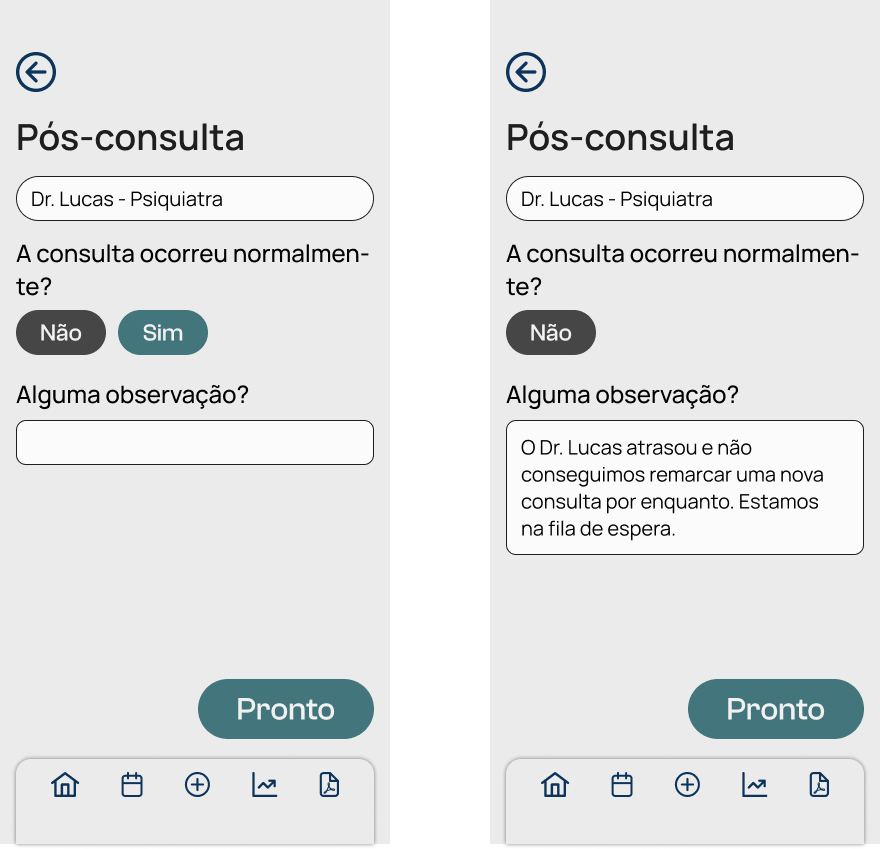
\includegraphics[width=1.0\linewidth]{assets/prototipo/Avaliação Consulta.png}
	\caption{Avaliação de Consulta}
	\fonte{Autores.}
	\label{avaliacao_consulta}
\end{figure}

\subsection{Calendário}

As telas de calendário foram projetadas para ajudar o usuário a visualizar e gerenciar suas consultas médicas de forma eficiente:

\begin{figure}[!htbp]
	\centering
	\includegraphics[width=0.6\linewidth]{assets/prototipo/Calendário - Consulta Finalizada-1.png}
	\caption{Calendário - Consulta Finalizada 1}
	\fonte{Autores.}
	\label{calendario_consulta_finalizada_1}
\end{figure}

\begin{figure}[!htbp]
	\centering
	\includegraphics[width=0.6\linewidth]{assets/prototipo/Calendário - Consulta Finalizada.png}
	\caption{Calendário - Consulta Finalizada}
	\fonte{Autores.}
	\label{calendario_consulta_finalizada}
\end{figure}

\begin{figure}[!htbp]
	\centering
	\includegraphics[width=0.6\linewidth]{assets/prototipo/Calendário.png}
	\caption{Calendário}
	\fonte{Autores.}
	\label{calendario}
\end{figure}

\subsection{Gráficos}

As telas de gráficos foram desenvolvidas para fornecer uma visualização clara e intuitiva dos dados de saúde do usuário:

\begin{figure}[!htbp]
	\centering
	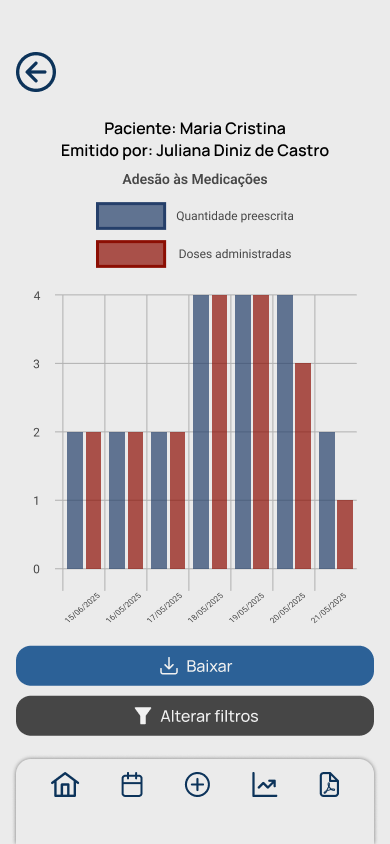
\includegraphics[width=0.6\linewidth]{assets/prototipo/Gráfico - Adesão a Medicações.png}
	\caption{Gráfico - Adesão a Medicações}
	\fonte{Autores.}
	\label{grafico_adesao_medicacoes}
\end{figure}

\begin{figure}[!htbp]
	\centering
	\includegraphics[width=0.6\linewidth]{assets/prototipo/Gráfico - Glicemia.png}
	\caption{Gráfico - Glicemia}
	\fonte{Autores.}
	\label{grafico_glicemia}
\end{figure}

\begin{figure}[!htbp]
	\centering
	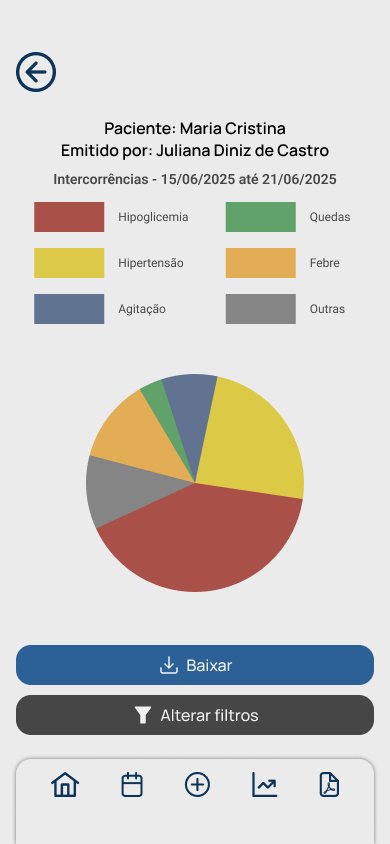
\includegraphics[width=0.6\linewidth]{assets/prototipo/Gráfico - Intercorrências.png}
	\caption{Gráfico - Intercorrências}
	\fonte{Autores.}
	\label{grafico_intercorrencias}
\end{figure}

\begin{figure}[!htbp]
	\centering
	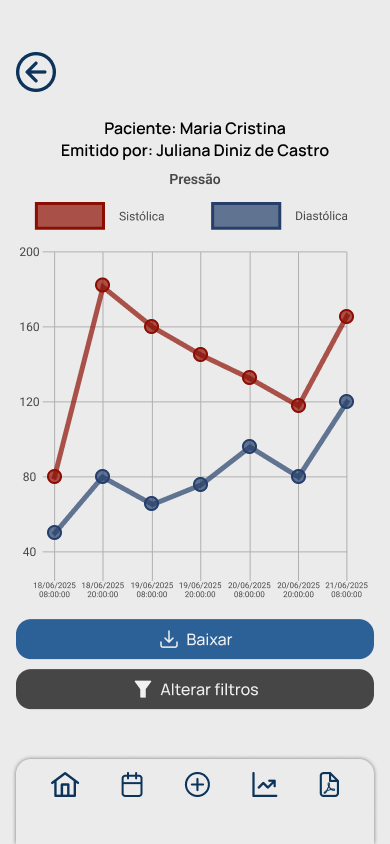
\includegraphics[width=0.6\linewidth]{assets/prototipo/Gráfico - Pressão.png}
	\caption{Gráfico - Pressão}
	\fonte{Autores.}
	\label{grafico_pressao}
\end{figure}

\begin{figure}[!htbp]
	\centering
	\includegraphics[width=0.6\linewidth]{assets/prototipo/Gráficos.png}
	\caption{Gráficos}
	\fonte{Autores.}
	\label{graficos}
\end{figure}

\subsection{Login e Perfil}

As telas de login e perfil foram projetadas para garantir uma experiência de usuário segura e personalizada:

\begin{figure}[!htbp]
	\centering
	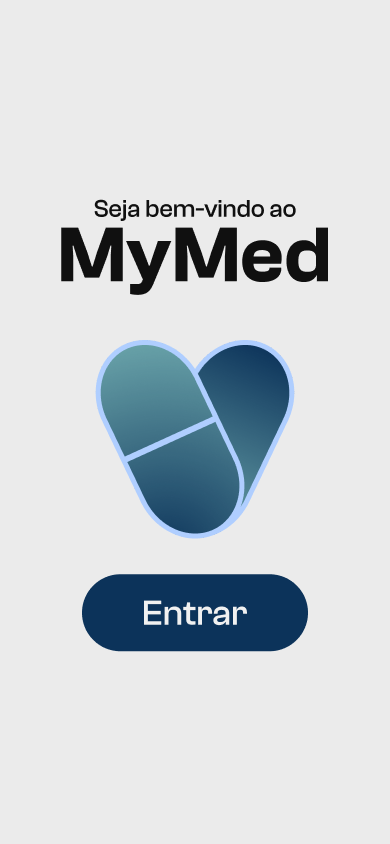
\includegraphics[width=0.6\linewidth]{assets/prototipo/Login.png}
	\caption{Login}
	\fonte{Autores.}
	\label{login}
\end{figure}

\begin{figure}[!htbp]
	\centering
	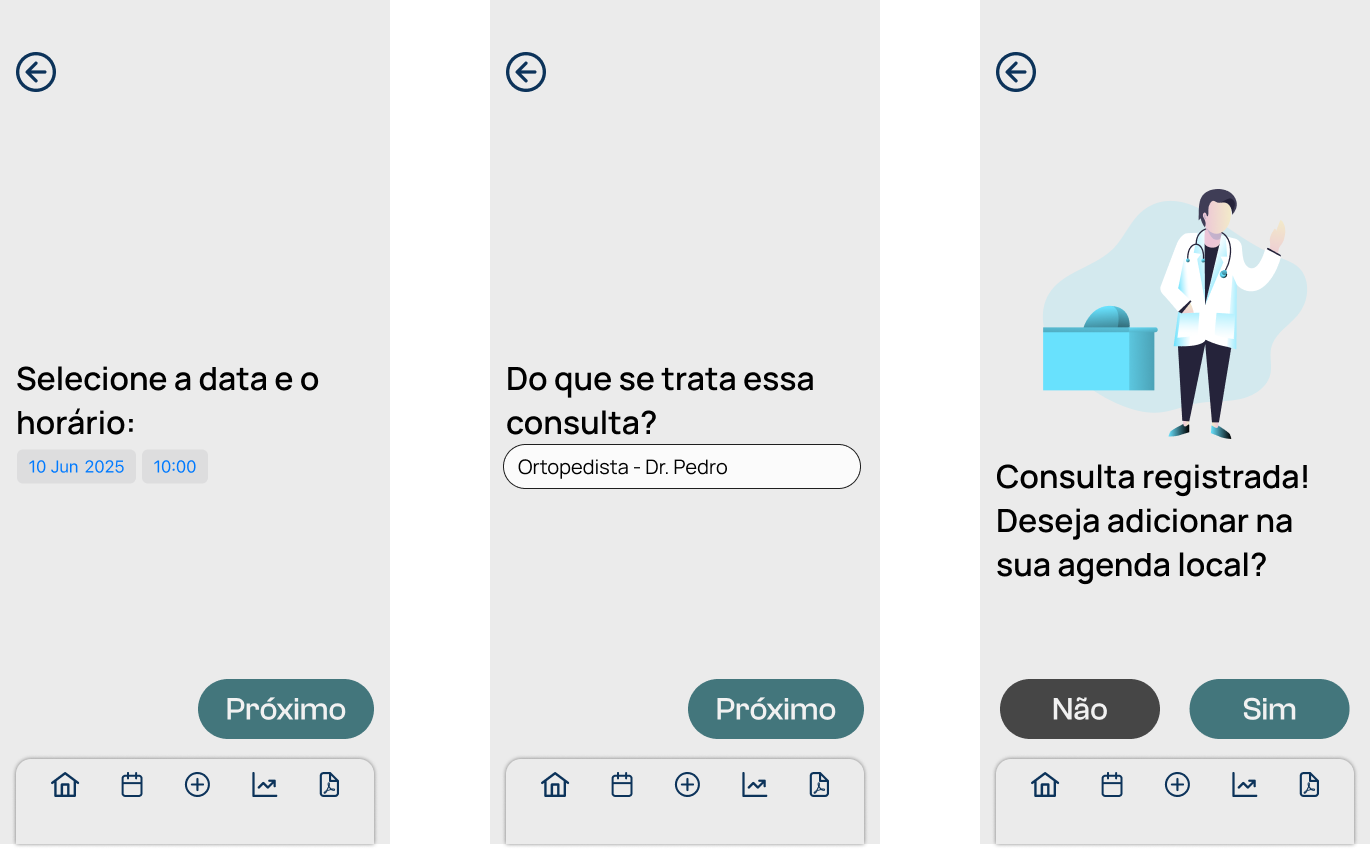
\includegraphics[width=1.0\linewidth]{assets/prototipo/Nova Consulta.png}
	\caption{Nova Consulta}
	\fonte{Autores.}
	\label{nova_consulta}
\end{figure}

\begin{figure}[!htbp]
	\centering
	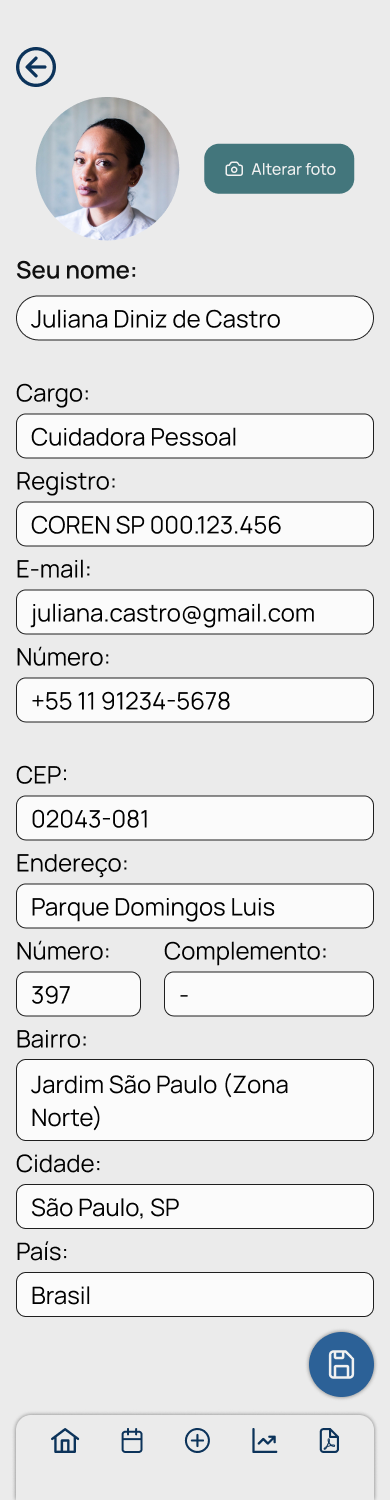
\includegraphics[width=0.35\linewidth]{assets/prototipo/Perfil - Edição.png}
	\caption{Perfil - Edição}
	\fonte{Autores.}
	\label{perfil_edicao}
\end{figure}

\begin{figure}[!htbp]
	\centering
	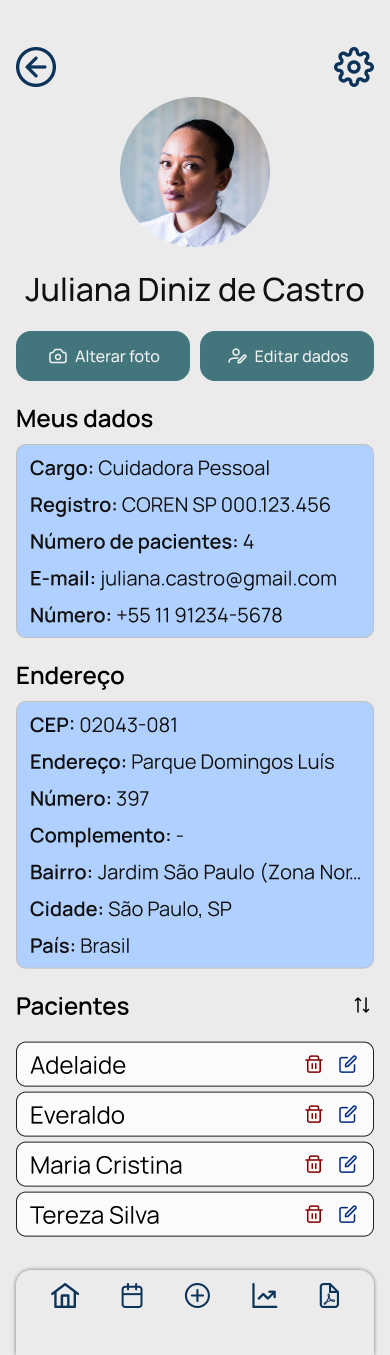
\includegraphics[width=0.35\linewidth]{assets/prototipo/Perfil.png}
	\caption{Perfil}
	\fonte{Autores.}
	\label{perfil}
\end{figure}

\begin{figure}[!htbp]
	\centering
	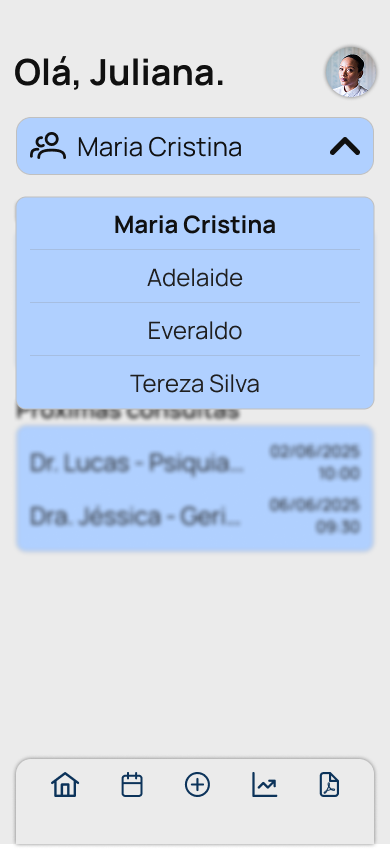
\includegraphics[width=0.6\linewidth]{assets/prototipo/Tela Inicial - Dropdown Nomes.png}
	\caption{Tela Inicial - Dropdown Nomes}
	\fonte{Autores.}
	\label{tela_inicial_dropdown_nomes}
\end{figure}

\subsection{Tela Inicial}

A tela inicial do aplicativo \nomeprojeto foi projetada para ser intuitiva e fácil de navegar, permitindo que os usuários acessem rapidamente as funcionalidades principais:

\begin{figure}[!htbp]
	\centering
	\includegraphics[width=0.6\linewidth]{assets/prototipo/Tela Inicial (Botão +).png}
	\caption{Tela Inicial (Botão +)}
	\fonte{Autores.}
	\label{tela_inicial_botao_mais}
\end{figure}

\begin{figure}[!htbp]
	\centering
	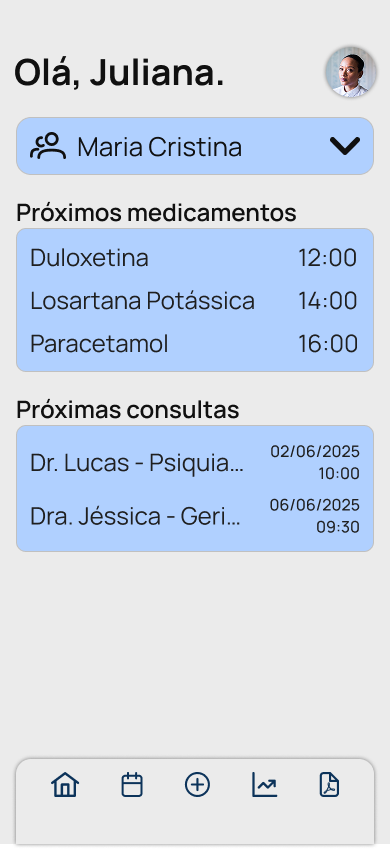
\includegraphics[width=0.6\linewidth]{assets/prototipo/Tela Inicial.png}
	\caption{Tela Inicial}
	\fonte{Autores.}
	\label{tela_inicial}
\end{figure}

\newpage

\chapter{Seção Empresa \label{secao_empresa}}
\setcounter{section}{0}
\section{Desenvolvimento de Estrutura Empresarial: Hyperion / MyMed}

\subsection*{Missão}
Queremos oferecer uma solução tecnológica eficiente e humanizada para auxiliar cuidadores, asilos e casas de repouso na organização e administração dos cuidados com idosos, promovendo segurança, bem-estar e qualidade de vida aos pacientes.

\subsection*{Visão}
Desejamos ser referência nacional no desenvolvimento de tecnologias voltadas ao cuidado de idosos, contribuindo para uma sociedade mais atenta, organizada e respeitosa com a terceira idade.  

\subsection*{Valores}
Responsabilidade - garantir o funcionamento confiável da plataforma, priorizando a segurança nas rotinas de medicação e cuidados.  

Cuidado - fornecer meios e ferramentas para garantir a segurança e uma melhora no gerenciamento e cuidado da saúde de idosos. 

\subsection*{Descrição da Empresa}
Nosso principal objetivo é desenvolver uma plataforma de auxílio de gerenciamento de tratamentos de um usuário e/ou seus dependentes, alertando sobre estoque remanescente, consultas agendadas, registros de índice de pressão e/ou glicemia. com um desenvolvimento próximo ao usuário final, interface simples e soluções razoáveis em comparação com a concorrência. 

\section{Análise de Mercado}

\subsection*{Público-Alvo (Personas)}
Cuidadores, geralmente cuidadores de pessoas da terceira idade, que passam seus dias de trabalho realizando tarefas exaustivas e que consomem grande parte do seu tempo.  O nome da nossa persona principal é Juliana. Juliana é uma cuidadora que trabalha em uma casa de repouso, onde ela tem quatro pacientes e está usando o MyMed para administrar o tratamento de seus pacientes, com enfoque em administrar as medicações e as consultas de cada paciente. 

\subsection*{Necessidades dos Usuários}
Uma melhor organização e gerenciamento dos tratamentos e medicações do paciente daquele cuidador, focando na centralização do monitoramento de recursos. Principalmente por conta de não existir programas de assistência aos cuidadores. 

Uma forma eficiente de guardar informações e emitir relatórios e acessar gráficos a partir de suas necessidades, como períodos, ocorrências e registros.

\subsection*{Concorrentes}
Medisafe:\\
 O que oferece de diferente: \\
- Gestão de medicamentos com lembretes e alertas. \\
- Compartilhamento básico de informações com familiares e cuidadores. \\
 Diferencial da sua aplicação: \\
-  Gráficos detalhados de adesão ao tratamento. \\
-  Análise de interações medicamentosas. \\
-  Recomendações personalizadas para o idoso e cuidador.\\

MyChart / SNS24:\\
 O que oferece de diferente: \\
- Agendamento e registro de consultas médicas.  \\
- Acesso a receitas e teleconsultas.\\
 Diferencial da sua aplicação: \\
-  Integração com sistemas locais de saúde.  \\
-  Análise preditiva de saúde.\\
-  Alertas personalizados para exames e consultas futuras. \\

Lively Mobile Plus / Lica:\\
 O que oferece de diferente:\\
-  Monitoramento de quedas e alertas emergenciais.\\
-  Monitoramento de sinais vitais em tempo real.\\
 Diferencial da sua aplicação:\\
-  Monitoramento contínuo com inteligência artificial para antecipar riscos.\\
-  Relatórios detalhados para familiares e cuidadores.\\

Hora do Lar / Américo Cuidador:\\
 O que oferece de diferente:\\
-  Gestão do cuidador profissional: contratação, controle de jornada e conformidade legal.\\
 Diferencial da sua aplicação:\\
-  Gestão integrada do idoso e do cuidador.\\
-  Dashboards multidimensionais que acompanham saúde, tarefas e bem-estar.\\

Cuidar de Idosos / Mais Amor Cuidadores:\\
 O que oferece de diferente:\\
-  Conteúdo educativo e dicas para cuidadores iniciantes.\\
 Diferencial da sua aplicação:\\
-  Conteúdo educativo integrado diretamente na plataforma.\\
-  Suporte em tempo real e canais de comunicação para dúvidas.\\

Apps de comunicação (ex: Hugs Care):\\
 O que oferece de diferente:\\
-  Troca de experiências entre cuidadores e familiares.\\
-  Comunicação simples e direta.\\
 Diferencial da sua aplicação:\\
-  Plataforma integrada para comunicação entre familiares, cuidadores e profissionais.\\
-  Histórico e notificações centralizadas para melhor acompanhamento.\\

DoseApp (código aberto):\\
 O que oferece de diferente:\\
-  Compartilhamento de informações sobre medicação e rotina.\\
-  Interface simples e acessível.\\
Diferencial da sua aplicação:\\
-  Interface intuitiva e multiplataforma (web e mobile).\\
-  Uso de inteligência artificial para personalização e automação de tarefas.\\
\subsection*{Diferenciais da Solução}
Temos como base do projeto o foco nos cuidadores, onde temos uma interface intuitiva, atraente e que centraliza as informações pertinentes aos pacientes, permitindo melhor compreensão do quadro do dependente, alertas e lembretes para melhor organização de tempo, relatórios personalizados sobre consultas e medicamentos, pesquisa de preços de medicamentos e desenvolvimento orientado à feedback do usuário. 

\section{Modelo de Negócio}
\begin{figure}[!htbp]
    \centering
    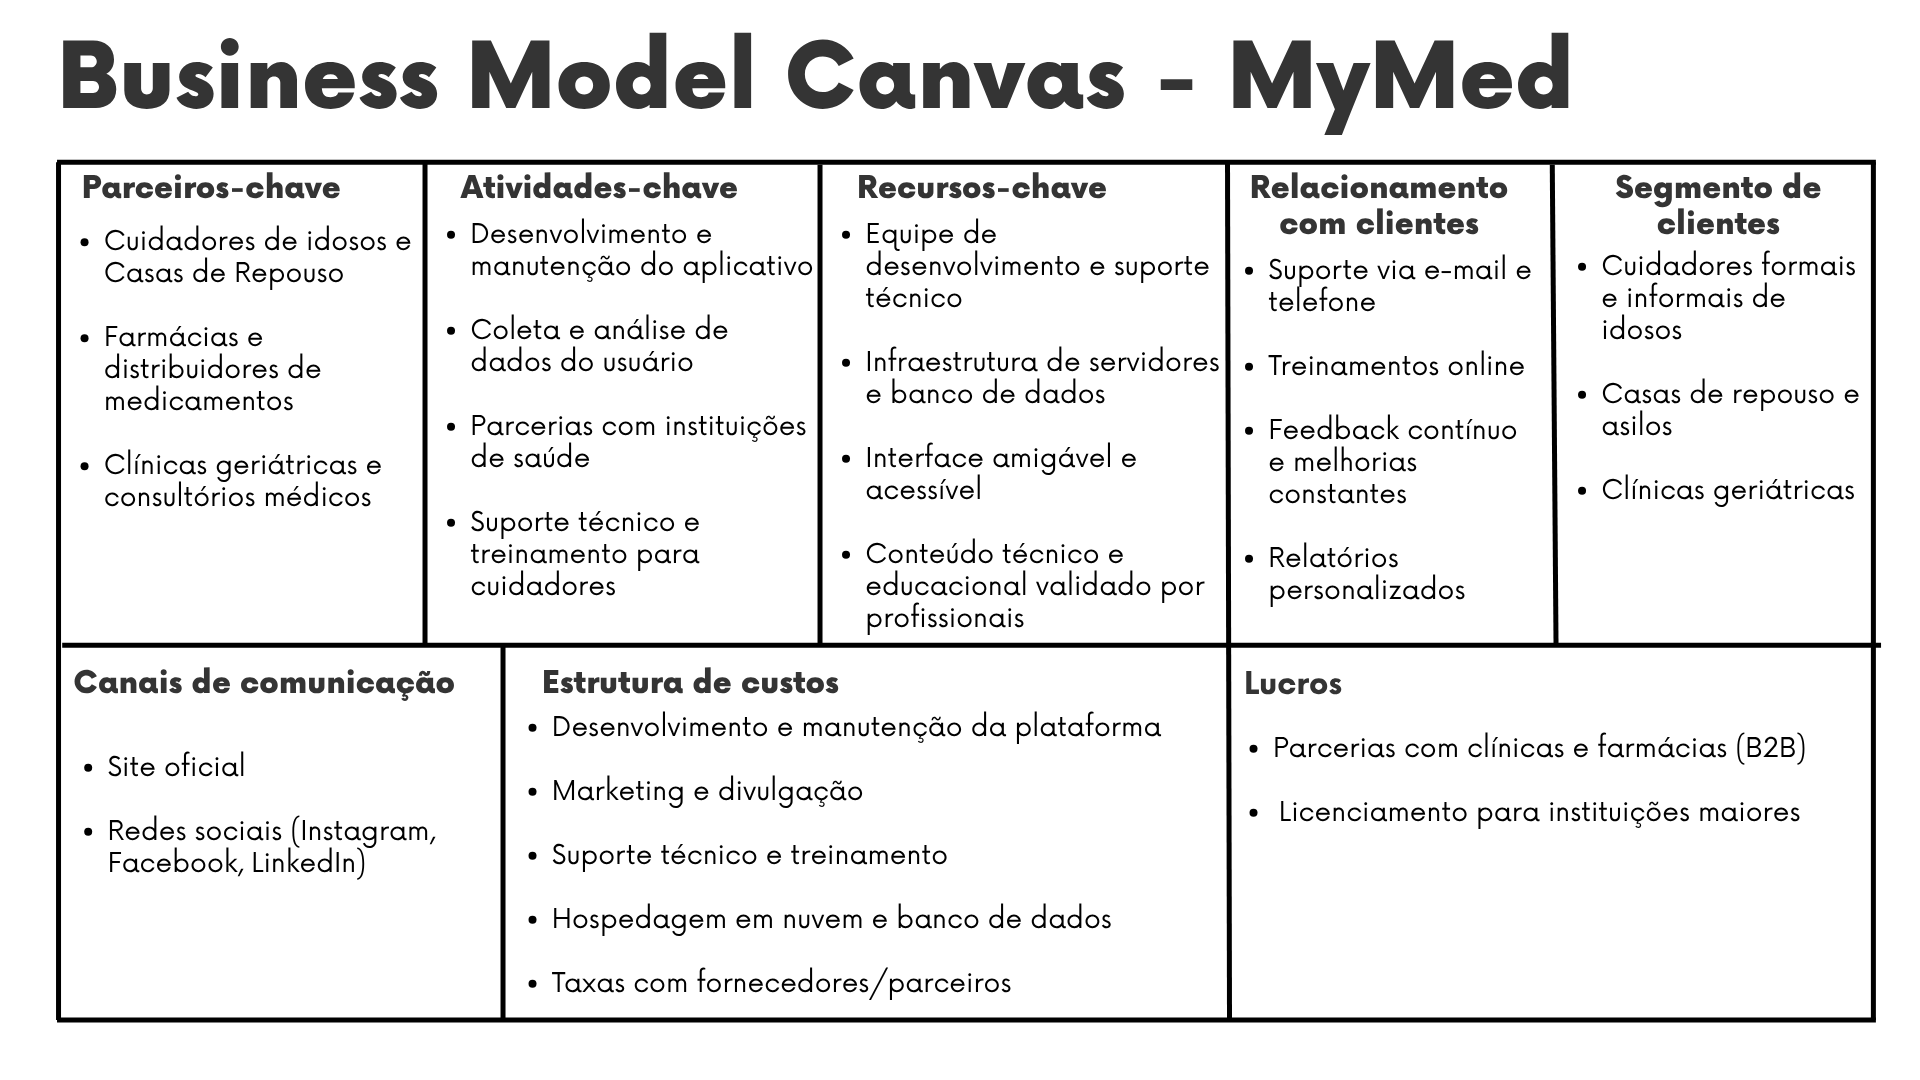
\includegraphics[width=0.75\linewidth]{assets/figuras/BMC.png}
    \caption{Business Model Canvas - MyMed}
    \fonte{Autores.}
\end{figure}

\subsection*{Fonte de Receita}
Nosso sistema tem enfoque em ser acessível e oferece uma versão gratuita com anúncios, alcançando um público amplo. Para uma experiência aprimorada, a assinatura Premium remove anúncios e desbloqueia funcionalidades avançadas que exigem uma maior análise de dados ou poder de processamento. Este modelo de assinatura é importante para a sustentabilidade do projeto, permitindo investimento contínuo em pesquisa, desenvolvimento e infraestrutura, garantindo um serviço inovador e de alta qualidade.

\subsection*{Parcerias Principais e Recursos-chave}
• Parcerias principais: Clínicas, farmácias, ONGs, planos de saúde, universidades;

• Recursos-chave: Equipe de desenvolvedores, Experiência do usuário (UX) acessível, base de dados segura, notificações e suporte ao usuário contínuo;

• Ativos estratégicos: Reputação, conteúdo educativo, comunidade ativa de cuidadores e divulgadores.

\section{Estratégia de Lançamento e Marketing}
No pré-lançamento, queremos disponibilizar uma versão beta do MyMed para familiarizar os usuários com a interface e estabelecer um canal contínuo de feedback para aprimoramento ao longo das próximas versões. A divulgação nesse período será realizada por meio de clínicas geriátricas, ONGs de saúde que trabalham com cuidadores e farmácias. A partir dos feedbacks, faremos uma análise se após aprimorar o projeto com as sugestões, podemos realizar o lançamento oficial, onde colocaremos o aplicativo nas lojas e disponibilizar o aplicativo para o público. Nosso foco no pós-lançamento é continuar investindo na pesquisa e desenvolvimento e aprimorar o aplicativo ao longo do tempo, com funcionalidades que mantenham o usuário engajado e fiéis ao nosso aplicativo. Nossas métricas de sucesso serão medidas através de número de downloads nas lojas de aplicativo, a retenção de usuários e o sucesso para realizar determinadas ações. 

Como estratégia de aquisição de usuários, realizaremos o marketing de conteúdo através de redes sociais, campanhas pagas de baixo custo (Google Ads), permitir o uso do aplicativo de forma gratuita para casas de repouso, cuidadores ou farmácias locais, e App Store Optimization (Play Store, App Store).

Nossos canais de divulgação serão as clínicas geriátricas, ONGs de saúde, farmácias (com material impresso simples como flyers com QR code), casas de repouso, redes sociais (principalmente Instagram), Google Ads e Facebook Ads, e, caso possível, influenciadores digitais (preferencialmente cuidadores).

\section{Aspectos Técnicos e Operacionais}

\subsection*{Tecnologias Utilizadas}
• Back-end: Java com SpringBoot, PostgreSQL, Render e Google Cloud.

• Front-end: Angular 19, PrimeNG, OAuth 2.0 e Firebase.

• Versionamento: Git, GitHub e GitKraken.

• Gestão: Jira e Google Drive.

\subsection*{Equipe e Funções}
A equipe e as funções de cada integrante são encontradas no \autoref{quadro_integrantes}.

\subsection*{Ferramentas de Desenvolvimento}
• Editor: Visual Studio Code.

• Versionamento: Git/GitHub.

• Gestão: Jira.

• Armazenamento: Google Drive.

\section{Viabilidade Econômica}

\subsection*{Custos Estimados}
Os custos estimados nos primeiros seis meses seriam de R\$50.000 a 60.000, considerando custos administrativos, marketing, servidores, design e desenvolvimento, mas se considerarmos que no início não teríamos um "salário" dignamente posto, o custo cairia para R\$35.000 a 45.000. 

\newpage

\chapter{Plano de Testes \label{plano_testes}}
\setcounter{section}{0}
\section{Plano de Testes}

O quadro apresenta o plano de testes do sistema, detalhando os principais objetos de teste e os critérios de sucesso para cada caso. Entre os itens testados estão a manutenção de usuários e admins, gestão de informações adicionais ao perfil, registro e consulta de pacientes, notificações de tratamento, pesquisa de farmácias e medicamentos, além do controle de registros de saúde como pressão arterial, glicose e adesão a medicamentos. Cada teste busca garantir a correta criação, edição, exclusão e visualização dos dados no sistema, assegurando o funcionamento esperado das funcionalidades essenciais para o gerenciamento de pacientes e seus tratamentos.

\begin{quadro}[!htbp]
    \caption{\label{quadro_plano_testes}Plano de Testes do Sistema}
    \small % Diminui a fonte para caber na página
    \begin{tabular}{|l|p{4cm}|p{5cm}|p{5cm}|}
        \hline
        \textbf{Código} & \textbf{Objeto de Teste} & \textbf{Sucesso} & \textbf{Erro} \\ \hline
        T01.1 & Criar usuário/admin & Criação de usuário ou admin no banco de dados & A conexão com o banco de dados pode falhar \\ \hline
        T01.2 & Editar usuário/admin & Edição de usuário ou admin no banco de dados & A conexão com o banco de dados pode falhar \\ \hline
        T01.3 & Excluir usuário/admin & Exclusão de usuário ou admin no banco de dados & A conexão com o banco de dados pode falhar \\ \hline
        T02.1 & Criar informações adicionais ao perfil de usuário & Adição de número de telefone, foto de perfil e endereço & A conexão com o banco de dados pode falhar; a foto de perfil pode apresentar erros de compressão \\ \hline
        T02.2 & Editar informações adicionais ao perfil de usuário & Edição de número de telefone, foto de perfil e endereço & A conexão com o banco de dados pode falhar; a foto de perfil pode apresentar erros de compressão \\ \hline
        T02.3 & Excluir informações adicionais ao perfil de usuário & Exclusão de número de telefone, foto de perfil e endereço & A conexão com o banco de dados pode falhar; a foto de perfil pode apresentar erros de compressão \\ \hline
        T03.1 & Criar paciente & Criação de paciente no banco de dados & A conexão com o banco de dados pode falhar \\ \hline
        T03.2 & Editar paciente & Edição de paciente no banco de dados & A conexão com o banco de dados pode falhar \\ \hline
        T03.3 & Excluir paciente & Exclusão de paciente no banco de dados & A conexão com o banco de dados pode falhar \\ \hline
        T04 & Enviar ao banco consulta de paciente & Criação de consulta no banco de dados & A conexão com o banco de dados pode falhar \\ \hline
        T05 & Visualizar consultas por dia/mês de paciente & Consultas organizadas pelo filtro de dia ou mês & A conexão com o banco de dados pode falhar; o conteúdo pode aparecer de forma errada \\ \hline
    \end{tabular}
    \fonte{Autores.}
\end{quadro}

\begin{quadro}[!htbp]
    \small
    \begin{tabular}{|l|p{4cm}|p{5cm}|p{5cm}|}
        \hline
        \textbf{Código} & \textbf{Objeto de Teste} & \textbf{Sucesso} & \textbf{Erro} \\ \hline
        T06 & Adicionar medicamento a um tratamento de paciente & Paciente consta que possui tratamento com aquele medicamento & A conexão com o banco de dados pode falhar \\ \hline
        T07 & Receber notificação de tratamento de paciente & Visualizar notificação de tratamento no horário que foi inserido & A notificação pode não aparecer; a notificação pode aparecer no horário errado; a notificação pode aparecer pertinente a outro paciente \\ \hline
        T08 & Manter atendimento de consulta de paciente & Criação, edição ou exclusão de atendimento de consulta & A conexão com o banco de dados pode falhar \\ \hline
        T09 & Pesquisar locais de farmácia & Visualizar farmácias nas proximidades & A conexão com a API pode falhar; o GPS do usuário pode estar desligado \\ \hline
        T10 & Pesquisar medicamentos de um determinado tratamento a venda & Visualizar a venda de medicamentos utilizados em tratamentos & A conexão com a API pode falhar \\ \hline
        T11 & Manter registro de pressão diastólica e sistólica de paciente & Criação, edição ou exclusão de gráfico de pressão cardiovascular & O gráfico pode apresentar erros em sua exibição; informações podem ser registradas erroneamente \\ \hline
        T12 & Manter registro de nível de glicose de paciente & Criação, edição ou exclusão de gráfico de nível glicose & O gráfico pode apresentar erros em sua exibição; informações podem ser registradas erroneamente \\ \hline
        T13 & Visualizar registro de adesão a medicamentos de paciente & Visualizar taxa de adesão de paciente a medicamentos & O gráfico pode apresentar erros em sua exibição; informações podem ser registradas automaticamente de forma errada \\ \hline
        T14 & Manter intercorrências de paciente & Criação, edição ou exclusão de intercorrências de paciente & O gráfico pode apresentar erros em sua exibição; informações podem ser registradas erroneamente \\ \hline
    \end{tabular}
    \fonte{Autores.}
\end{quadro}


\end{apendicesenv}

% % ----------------------------------------------------------
% % Anexos
% % ----------------------------------------------------------
% \cftinserthook{toc}{AAA}
% % ---
% % Inicia os anexos
% % ---
% %\anexos
% \newpage
% \begin{anexosenv}

% % ---
% \chapter{Cras non urna sed feugiat cum sociis natoque penatibus et magnis dis
% parturient montes nascetur ridiculus mus}
% % ---

% Anexos são os documentos não elaborados pelo autor, que servem de fundamentação, comprovação ou ilustração, como mapas, leis, estatutos etc.

% Os apêndices devem aparecer após as referências, e os anexos, após os apêndices.

% \end{anexosenv}

\end{document}
